% !TEX program = xelatex
\documentclass[a4paper]{article}

%%%%%%%% CREATE DOCUMENT STRUCTURE %%%%%%%%
%% Language and font encodings
\usepackage[english]{babel}
\usepackage[utf8x]{inputenc}
\usepackage[T1]{fontenc}
%\usepackage{subfig}

%% Sets page size and margins
\usepackage[a4paper,top=3cm,bottom=2cm,left=2cm,right=2cm,marginparwidth=1.75cm]{geometry}

%% Useful packages
\usepackage{amsmath}
\usepackage{wasysym}
\usepackage{graphicx}
\usepackage[colorinlistoftodos]{todonotes}
\usepackage[colorlinks=true, allcolors=blue]{hyperref}
\usepackage{caption}
\usepackage{subcaption}
\usepackage{sectsty}
\usepackage{float}
\usepackage{titling} 
\usepackage{siunitx}
\usepackage{listings}
\usepackage{blindtext}
\usepackage[square,sort,comma,numbers]{natbib}
\usepackage{tcolorbox}
\usepackage[colorinlistoftodos]{todonotes}
\usepackage{xcolor}
\usepackage{nicefrac}
\definecolor{darkgreen}{rgb}{0.0, 0.4, 0.0}
\sisetup{
    separate-uncertainty = true,  % Display uncertainty with \pm
    output-decimal-marker = {.},  % Ensure decimal point is a dot
}

\lstdefinestyle{CStyle}{
    language=C,
    frame=single,
    numbers=left,
    numberstyle=\tiny,
    basicstyle=\ttfamily\footnotesize,
    keywordstyle=\color{blue},
    commentstyle=\color{green!50!black},
    stringstyle=\color{red},
    tabsize=4,
    showspaces=false,
    showstringspaces=false,
    breaklines=true,
    breakatwhitespace=true,
    captionpos=b
}

% Define a gray example box
\tcbset{
    examplebox/.style={
        colback=gray!10,  % Background color
        colframe=gray,    % Border color
        fonttitle=\bfseries,
        title=Example,    % Default title for the box
        sharp corners,
        boxrule=0.5mm,    % Border thickness
        coltitle=black,   % Title color
    }
}
%%% Stuff for code
\definecolor{codegreen}{rgb}{0,0.6,0}
\definecolor{codegray}{rgb}{0.5,0.5,0.5}
\definecolor{codepurple}{rgb}{0.58,0,0.82}
\definecolor{backcolour}{rgb}{0.95,0.95,0.92}
\lstdefinestyle{mystyle}{
    backgroundcolor=\color{backcolour},   
    commentstyle=\color{codegreen},
    keywordstyle=\color{magenta},
    numberstyle=\tiny\color{codegray},
    stringstyle=\color{codepurple},
    basicstyle=\ttfamily\footnotesize,
    breakatwhitespace=false,         
    breaklines=true,                 
    captionpos=b,                    
    keepspaces=true,                 
    numbers=left,                    
    numbersep=5pt,                  
    showspaces=false,                
    showstringspaces=false,
    showtabs=false,                  
    tabsize=2
}
%no indent after new line!
\setlength{\parindent}{0pt}
\lstset{style=mystyle}

\newcommand{\TODO}[1]{\textcolor{red}{TODO: \textbf{#1\\}}}
\newcommand{\Shining}[1]{\textcolor{cyan}{\textbf{#1}}}
%%%%
\renewcommand\thesubsection{\thesection.\alph{subsection})}

%%%%%%%% DOCUMENT %%%%%%%%
\begin{document}

%%%% Title Page
\begin{titlepage}

\newcommand{\HRule}{\rule{\linewidth}{0.5mm}} 							% horizontal line and its thickness
\center 
 
% University
\textsc{\LARGE Delft University of Technology}\\[1cm]

% Document info
\textsc{\Large Introduction to High Performance Computing}\\[0.2cm]
\textsc{\large WI4049TU}\\[1cm] 										% Course Code
\HRule \\[0.8cm]
{ \huge \bfseries Lab Report}\\[0.7cm]								% Assignment
\HRule \\[2cm]
\large
\emph{Author:}\\
Elias Wachmann (6300421) \\[1.5cm]
{\large \today}\\[5cm]

\includegraphics[width=0.6\textwidth]{../fig/TU_delft_logo.jpg}\\[1cm] 	% University logo
\vfill 
\end{titlepage}
\input{input/general\_remarks.tex}
\setcounter{section}{-1}
\section{Introductory exercise}
In the introductory lab session, we are taking a look at some basic features of MPI. 

We start out very simple with a hello world program on two nodes. 

\subsection*{Hello World}
\lstinputlisting[language=c]{input/code/00/helloworld1.c}
This program can be compiled with the following command:\\

\begin{verbatim}
mpicc -o helloworld1.out helloworld1.c
\end{verbatim}
And run with:
\begin{verbatim}
srun -n 2 -c 4 --mem-per-cpu=1GB  ./helloworld1.out
\end{verbatim}
We get the following output:
\begin{verbatim}
Node 0 of 2 says: Hello world!
Node 1 of 2 says: Hello world!
\end{verbatim}

From now on I'll skip the compilation and only mention on how many nodes the program is run and what the output is / interpretation of the output.

\subsection{Ping Pong}
I used the template to check how long \texttt{MPI\_Send} and \texttt{MPI\_Recv} take. The code can be found in the appendix for this section. \\

I've modified the printing a bit to make it easier to gather the information. 
Then I piped the program output into a textfile for further processing in python. I ran it first on one and then on two nodes as specified in the assignment sheet. Opposed to the averaging over 5 send / receive pairs, I've done 1000 pairs. Furthmore I reran the whole programm 5 times to gather more data. 
All this data is shown in the following graph: 
% add figure
\begin{figure}[H]
    \centering
    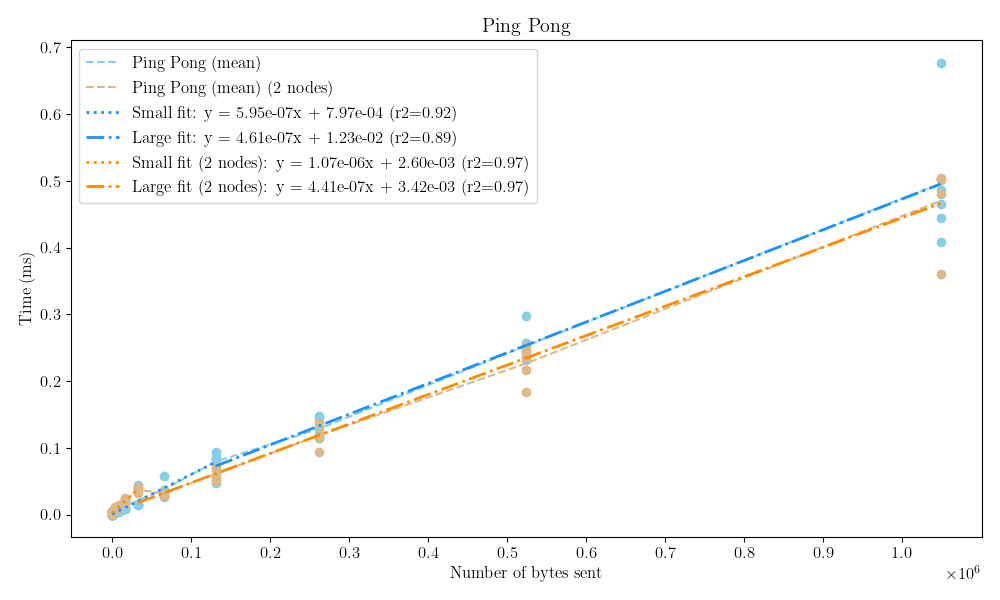
\includegraphics[width=\textwidth]{../fig/lab0/pingPong.png}
    \caption{Ping Pong: Number of bytes sent vs. average time taken from 1000 pairs of send / receive. 5 runs shown for each size as scatter plot. Mean of these 5 runs shown as line. Blue small fit includes all data points up to 131072 bytes, blue large from there. Red small fit includes all data points up to 32768 bytes, red large from there.}
    \label{fig:pingpong}
\end{figure}
As can be seen in the data and the fits, there are outliers especially for the larger data sizes. \\
For our runs we get the following fits and $R^2$ values:
\begin{table}[h!]
    \centering
    \begin{tabular}{|l|l|l|l|}
        \hline
        \textbf{Run Type}   & \textbf{Data Size} & \textbf{Fit Equation}                                      & \textbf{$R^2$ Value} \\ \hline
        \textbf{Single Node} & Small (<=131072)             & $5.95 \times 10^{-7} \cdot x + 7.97 \times 10^{-4}$        & 0.92              \\ \hline
        \textbf{Single Node} & Large (>= 131072)& $4.61 \times 10^{-7} \cdot x + 1.23 \times 10^{-2}$        & 0.89              \\ \hline
        \textbf{Two Node}    & Small (<=32768)& $1.07 \times 10^{-6} \cdot x + 2.60 \times 10^{-3}$        & 0.97              \\ \hline
        \textbf{Two Node}    & Large (>=32768)   & $4.41 \times 10^{-7} \cdot x + 3.42 \times 10^{-3}$        & 0.97              \\ \hline
    \end{tabular}
    \caption{Fit Equations and $R^2$ Values for Single Node and Two Node Runs}
\end{table}

\Shining{Note:} Each run was performed 5 times (for 1 and 2 nodes) to get a fit on the data and calculate a $R^2$ value. 

\subsubsection*{\Shining{Extra: Ping Pong with MPI\_SendRecv}}
We do the same analysis for the changed program utilizing \texttt{MPI\_SendRecv}. The code can be found in the appendix for this section. \\
We get the following graph from the measurements which were performed in the same way as for the previous program:
% add figure
\begin{figure}[H]
    \centering
    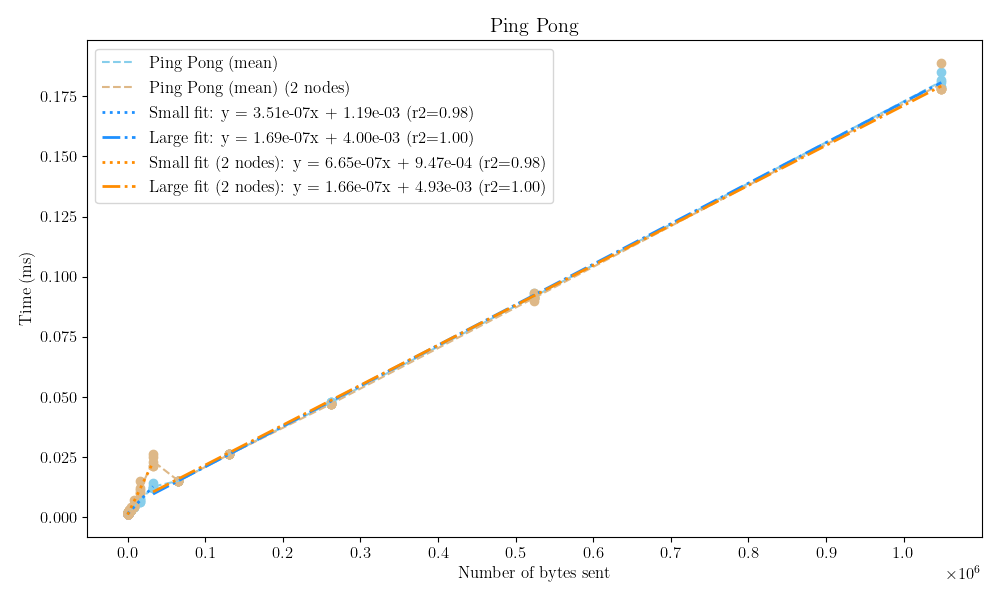
\includegraphics[width=\textwidth]{../fig/lab0/pingPongSR.png}
    \caption{Ping Pong with MPI\_SendRecv: Number of bytes sent vs. average time taken from 1000 pairs of send / receive. 5 runs shown for each size as scatter plot. Mean of these 5 runs shown as line. Blue small fit includes all data points up to 32768 bytes, blue large from there. Red small fit includes all data points up to 32768 bytes, red large from there.}
    \label{fig:pingpongSendRecv}
\end{figure}

We get the following fits and $R^2$ values for the runs:
\begin{table}[h!]
    \centering
    \begin{tabular}{|l|l|l|l|}
        \hline
        \textbf{Run Type}   & \textbf{Data Size} & \textbf{Fit Equation}                                      & \textbf{$R^2$ Value} \\ \hline
        \textbf{Single Node} & Small (<=32768)  & $3.51 \times 10^{-7} \cdot x + 1.19 \times 10^{-3}$        & 0.98              \\ \hline
        \textbf{Single Node} & Large (>=32768)  & $1.69 \times 10^{-7} \cdot x + 4.00 \times 10^{-3}$        & 1.00              \\ \hline
        \textbf{Two Node}    & Small (<=32768)  & $6.65 \times 10^{-7} \cdot x + 9.47 \times 10^{-4}$        & 0.98              \\ \hline
        \textbf{Two Node}    & Large (>=32768)  & $1.66 \times 10^{-7} \cdot x + 4.93 \times 10^{-3}$        & 1.00              \\ \hline
    \end{tabular}
    \caption{Fit Equations and $R^2$ Values for Single Node and Two Node Runs}
\end{table}


\subsection{MM-product}
After an introduction of the matrix-matrix multiplication code in the next section, the measured speedups are discussed in the subsequent section.
\subsubsection*{Explanation of the code}
For this excercise I've used the template provided in the assignment sheet as a base to develop my parallel implementation for a matrix-matrix multiplication. The code can be found in the appendix for this section. \\

The porgam can be run either in sequential (default) or parallel mode (parallel as a command line argument). For the sequential version, the code is practically unchanged and just refactored into a function for timing purposes. The parallel version is more complex and works as explained bellow: \\
First, rank 0 computes a sequential reference solution. Then rank 0 distributes the matrices in the following way in \texttt{splitwork}: 
\begin{itemize}
    \item Matrix A is split row-wise by dividing the number of rows by the number of nodes.
    \item The first worker (=rank 1) gets the most rows starting from row 0: \\$\texttt{total\_rows} - (\texttt{nr\_workers}-1) \cdot \textit{floor}(\frac{\texttt{total\_rows}}{\texttt{nr\_workers}})$.
    \item All other workers and the master (= rank 0) get the same number of rows: $\textit{floor}(\frac{\texttt{total\_rows}}{\texttt{nr\_workers}})$.
    \item The master copies the corresponding rows of matrix A and the whole transposed matrix B\textcolor{cyan}{\textbf{*}} into a buffer (for details on \texttt{MM\_input} buffer see bellow) for each worker and sends them off using \texttt{MPI\_ISend}.
    \item The workers receive the data using \texttt{MPI\_Recv} and then compute their part of the matrix product and send only the rows of the result matrix back to the master using \texttt{MPI\_Send}.
    \item In the meanwhile the master computes its part of the matrix product.
    \item Using \texttt{MPI\_Waitall} the master waits for all data to be sent to the workers and only afterwards calls \texttt{MPI\_Recv} to gather the results from the workers.
    \item Finally all results are gathered by the master in the result matrix.
\end{itemize}
Assume we have a 5x5 matrix $A$ and 2 workers (rank 1 and rank 2) and master (rank 0). The partitioning is done row-wise as follows:
\begin{tcolorbox}[examplebox, title=Partitioning Example]

\[
A =
\begin{pmatrix}
    a_{11} & a_{12} & a_{13} & a_{14} & a_{15} \\
    a_{21} & a_{22} & a_{23} & a_{24} & a_{25} \\
    a_{31} & a_{32} & a_{33} & a_{34} & a_{35} \\
    a_{41} & a_{42} & a_{43} & a_{44} & a_{45} \\
    a_{51} & a_{52} & a_{53} & a_{54} & a_{55} \\
\end{pmatrix} \rightarrow
\begin{pmatrix}
    \text{Worker 1} \\
    \text{Worker 1} \\
    \text{Worker 1} \\
    \text{Master} \\
    \text{Master} \\
\end{pmatrix}
\]

\begin{itemize}
    \item \textbf{Rank 0 (Master)}: Rows 4 and 5 (last two rows)
    \item \textbf{Rank 1 (Worker 1)}: Rows 1 to 3 (first three rows) - Worker 1 always gets the most rows
\end{itemize}

This partitioning can be visually represented as:

\[
\text{Master (rank 0):}
\begin{pmatrix}
    a_{41} & a_{42} & a_{43} & a_{44} & a_{45} \\
    a_{51} & a_{52} & a_{53} & a_{54} & a_{55} \\
\end{pmatrix}
\]

\[
\text{Worker 1 (rank 1):}
\begin{pmatrix}
    a_{11} & a_{12} & a_{13} & a_{14} & a_{15} \\
    a_{21} & a_{22} & a_{23} & a_{24} & a_{25} \\
    a_{31} & a_{32} & a_{33} & a_{34} & a_{35} \\
\end{pmatrix}
\]

\end{tcolorbox}
Each worker computes its part of the matrix product, and the master gathers the results at the end and compiles them into the final matrix.

The \texttt{MM\_input} buffer is used to store the rows of matrix A and the whole matrix B for each worker. It is implemented using a simple struct:
\begin{lstlisting}[language=c]
typedef struct MM_input {
    size_t rows;
    double *a;
    double *b;
} MM_input;
\end{lstlisting}

\Shining{*[Optimization] Note on transposed matrix B:} It is usually beneficial from a cache perspective to index arrays sequentially or in a row-major order. However, in the matrix-matrix multiplication, we access the elements of matrix B in a column-wise order. This leads to cache misses and is not optimal. To mitigate this, we can transpose matrix B and then access it in a row-wise order. This is done in the code by the master before sending the data to the workers.

\subsubsection*{Discussion of the speedups}
The code was run on Delft's cluster with 1, 2, 4, 8, 16, 24, 32, 48, and 64 nodes. For the experiments the matrix size of $A$ and $B$ was set to $2000\times2000$. 
This means that the program has to evaluate $2000$ multiplications and $1999$ additions for each element of the resulting matrix $C$. In total this results in $\approx 2000^3 = 8 \times 10^9$ operations.\\
The command looked similar to the following for the different node counts:
\begin{verbatim}
srun -n 48 --mem-per-cpu=4GB --time=00:02:00 ./MM.out parallel
\end{verbatim}
For this experiment, the execution time was measured and the speedup was calculated. The results are shown in \autoref{tab:execution_time} and \autoref{fig:speedup}.

\begin{table}[h!]
    \centering
    \begin{tabular}{|c|c|c|}
        \hline
        \textbf{CPU Count} & \textbf{Execution Time / s} & \textbf{Approx. Speedup} \\ 
        \hline
        1   & 47.11  & 1.0 \\ 
        2   & 10.26  & 4.6 \\ 
        4   & 10.30  & 4.6 \\ 
        8   &  5.20  & 9.1 \\ 
        16  &  2.97  & 15.9 \\ 
        24  &  2.54  & 18.5 \\ 
        32  &  2.29  & 20.6 \\ 
        48  &  2.98  & 15.8 \\ 
        64  &  1.72  & 27.4 \\ 
        \hline
    \end{tabular}
    \caption{Execution Time vs CPU Count}
    \label{tab:execution_time}
\end{table}

\begin{figure}[H]
    \centering
    \includegraphics[width=0.8\textwidth]{../fig/lab0/MM\_plot.png}
    \caption{Speedup vs CPU Count\\
    Black $\times$ marks the average of the rerun for $n=48$.}
    \label{fig:speedup}
\end{figure}

\Shining{Note:} The speedup is calculated as $S = \frac{T_1}{T_p}$, where $T_1$ is the execution time on 1 node and $T_p$ is the execution time on $p$ nodes.\\

\textbf{Discussion:}\\
As one can cleary discern from the data in \autoref{tab:execution_time} and \autoref{fig:speedup}, the speedup increases with the number of nodes (with the exception of $n=48$). This is expected as the more nodes we have, the more work can be done in parallel. However, the speedup is not linear. This is due to the overhead of communication between the nodes. The more nodes we have, the more communication is needed, and this overhead increases. This is especially visible in the data for $n=48$. Here the speedup is lower than for $n=32$. For this run the communication didn't went as smooth as for the other runs. This can potentially be attributed to the fact that one (or more) of the nodes or the network was under heavy load during this task. \\

\Shining{[Further investigation]} After observing this slower speed for the $n=48$, I reran the tests multiple times and got a runtime of around $1.9 s$ which was to be expected initially. Therefore, this one run is an odd one out, most likely due to the reasons mentioned above! I've also added the averaged data of the reruns as a datapoint in \autoref{fig:speedup}.\\
Another interesting fact can be seen when comparing the time taken for $n=1$ and $n=2$. They don't at all scale with the expected factor of 2. This is could be due to the fact, that the resource management system prefers runs with multiple nodes instead of a single node (= sequential). \\

Additional notes: The flag \texttt{--mem-per-cpu=<\#>GB} was set depending on the number of nodes used. For 1-24 nodes 8GB was used, for 32-48 nodes 4GB, and for 64 nodes 3GB. This had to be done to comply with QOS policy on the cluster. 

% \TODO{Data locality?}









\newpage
\section{Poisson solver}
\label{sec:poisson}
\renewcommand{\thesubsection}{\thesection.\arabic{subsection}}
In this section of the lab report, we will dicuss a prallel implementation of the Poisson solver. The Poisson solver is a numerical method used to solve the Poisson equation, which is a partial differential equation that is useful in many areas of physics. \\
\textbf{Note:} For local testing and development I'll run the code with \texttt{mpirun} instead of the \texttt{srun} command on the cluster. \\

\subsection{Building a parallel Poisson solver}
For the first part of the exercise we follow the steps lined out in the assignment sheet. I'll comment on the steps 1 through 10 and related questions bellow. The finished implementation can be found in the appendix for this section. \\
\begin{enumerate}
    \item \textbf{Step:} After adding MPI\_Init and MPI\_Finalize, we can run the program with multiple processes. We can see that the program runs with 4 processes in \autoref{fig:poisson_step1} via the quadrupeled output.
    \begin{figure}[H]
        \centering
        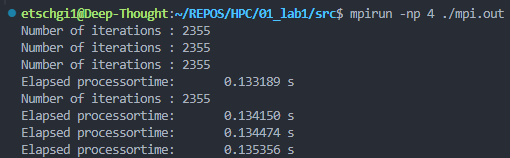
\includegraphics[width=0.5\textwidth]{../fig/lab1/step1.png}
        \caption{MPI\_Poisson after Step 1 - Running with 4 processes}
        \label{fig:poisson_step1}
    \end{figure}
    \item \textbf{Step:} To see which process is doing what, I included the rank of the process for the print statements as shown in \autoref{fig:poisson_step2}.
    \begin{figure}[H]
        \centering
        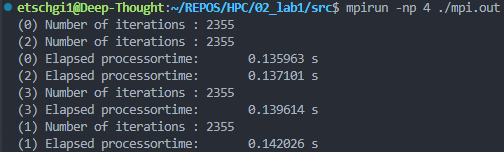
\includegraphics[width=0.5\textwidth]{../fig/lab1/step2.png}
        \caption{MPI\_Poisson after Step 2 - Running with 4 processes}
        \label{fig:poisson_step2}
    \end{figure}
    \item \textbf{Step:} Next we define \texttt{wtime} as a global double and replace the four utility timing functions with the ones given on Brightspace. A quick verification as shown in \autoref{fig:poisson_step3} shows that the program still runs as expected.
    \begin{figure}[H]
        \centering
        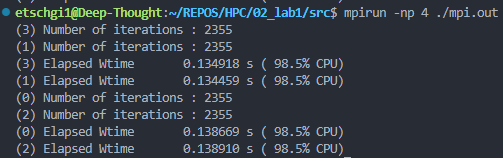
\includegraphics[width=0.5\textwidth]{../fig/lab1/step3.png}
        \caption{MPI\_Poisson after Step 3 - Running with 4 processes}
        \label{fig:poisson_step3}
    \end{figure}
    \item \textbf{Step:} Next we check if two processes indeed give the same output. Both need 2355 iterations to converge and the \texttt{diff} command returned no output, which means that the files content is identical. 
    \item \textbf{Step:} Now only the process with rank 0 will read data from files and subsequently broadcast it to the others. Testing this again with 2 processes, we see an empty diff of the output files and the same number of iterations needed to converge.
    \item \textbf{Step:} We create a cartesian grid of processes using \texttt{MPI\_Cart\_create} and use \texttt{MPI\_Cart\_shift} to find the neighbors of each process. We can see that the neighbors are correctly identified in \autoref{fig:poisson_step6}. 
    \begin{figure}[H]
        \centering
        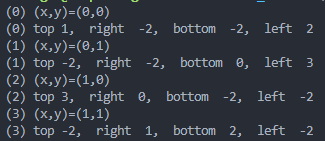
\includegraphics[width=0.5\textwidth]{../fig/lab1/step6.png}
        \caption{MPI\_Poisson after Step 6 - Running with 4 processes on a 2x2 grid}
        \label{fig:poisson_step6}
    \end{figure}
    When there is no neighbor in a certain direction, -2 (or \texttt{MPI\_PROC\_NULL}) is returned. 
    \item \textbf{Step:} We overhaul the setup to get a proper local grid for each process. Furthermore, we only save the relevant source fields in the local grid for each process. \\
    \Shining{With for instance 3 processes you should see that 1 or 2 processes do not do any 
    iteration. Do you understand why?}\\
    If we have a look at the input file we see that there are only 3 source fields in the grid. This means that the process that does not have a source field in its local grid will not do any iterations (or only 1). Therefore, if we have 3 processes and the distribution of source fields as given in the input file only 1 process will do iterations if processes are ordered in x-direction and 2 if ordered in y-direction. From this we can conclude that indeed all processes have different local grids and perform different calculations. 
    \begin{figure}[H]
        \centering
        \begin{minipage}{0.48\textwidth}
            \centering
            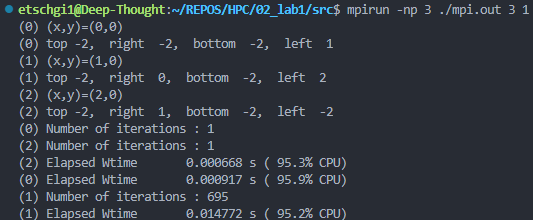
\includegraphics[width=\linewidth]{../fig/lab1/step7a.png}
        \end{minipage}%
        \hspace{0.02\textwidth}
        \begin{minipage}{0.48\textwidth}
            \centering
            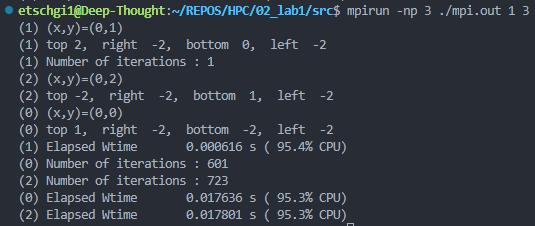
\includegraphics[width=\linewidth]{../fig/lab1/step7b.png}
        \end{minipage}
        \caption{MPI\_Poisson after Step 7 - Running with 3 processes on a 3x1 (left) vs. 1x3 (right) grid\\For the 3x1 grid, only rank 1 does iterations ($> 1$), for the 1x3 grid, ranks 0 and 2 do iterations ($> 1$).}
        \label{fig:poisson_step7}
    \end{figure}
    \item \textbf{Step:} After defining and commiting two special datatypes for vertical and horizontal communication, we setup the communication logic to exchange the boundary values between the processes. We call our \texttt{Exchange\_Borders} function after each iteration (for both red / black grid points). Now we face the problem in which some processes may stop instantly (no source in their local grid). They will not supply any data to their neighbors, which will cause the program to hang. We shall fix this in the next step.
    \item \textbf{Step:} Finally we need to implement the logic to check for convergence (in a global sense). We do this by using a \texttt{MPI\_Allreduce} call with the \texttt{MPI\_MAX} operation. This way we aggregate all deltas and choose the biggest one for the global delta which we use in the while-loop-condition to check for convergence. We can see that the program now runs as expected in \autoref{fig:poisson_step9}.
    \begin{figure}[H]
        \centering
        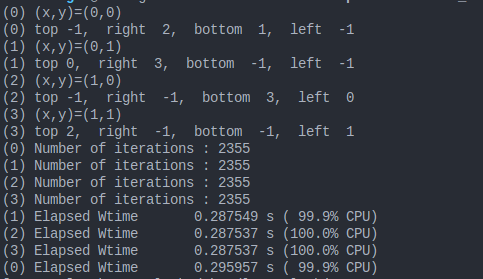
\includegraphics[width=0.5\textwidth]{../fig/lab1/step9.png}
        \caption{MPI\_Poisson after Step 9 - Running with 4 processes on a 2x2 grid}
        \label{fig:poisson_step9}
    \end{figure}
    Note that this run in \autoref{fig:poisson_step9} was done with another pc and another MPI implementation. Therefore, we see $-1$ for cells without a neighbor! However, other than that cosmetic difference it has no impact on the programm. 
    \item \textbf{Step:} Now we only have to fix two remaining things. First we have to make sure that each process uses the right global coordinates for the output file in the end. Therefore, we change the function a bit to include the specific x-/y-offset for each processor. The second thing is the potential problem, that different processors might start with different (red/black) parities. In order to accomplish a global parity we simply have to change the calculation in the if in \texttt{Do\_Step} from 
    \begin{lstlisting}[language=c, lastline=1]
        if ((x + y) % 2 == parity && source[x][y] != 1)
    \end{lstlisting}
    to
    \begin{lstlisting}[language=c, lastline=1]
        if ((x + offset[X_DIR] + y + offset[Y_DIR]) % 2 == parity && source[x][y] != 1)
    \end{lstlisting}
    this guarantees that during a given iteration all processors are using the same parity. 
\end{enumerate}
This just leaves one question open: Are the results acutally the same?\\
Checking the output files of the MPI-implementation with the sequential reference indeed shows identical numerical values for the calculated points. Furthermore, the needed iterationcount is also identical which isn't a big surprise, given that the two programms perform the exact same calculation steps. 

\subsection{Exercises, modifications, and performance aspects}
For this subsection we'll define the following shorthand notation: \\
\begin{table}[h!]
    \centering
    \caption{Notation for this section}
    \begin{tabular}{|l|l|}
        \hline
        $n$:  &the number of iterations\\\hline
        $g$:  &gridsize\\\hline
        $t$:  &time needed in seconds\\\hline
        $pt$: & processor topology in form $pxy$, where:\\
        $p$:  &number of processors used\\
        $x$:  &number of processors in x-direction\\
        $y$:  &number of processors in y-direction\\\hline
       \end{tabular}
\end{table}
$pt = 414$ means 4 processors in a $1\times 4$ topology. \\

\textbf{Note on different Versions:}\\
For the following exercises the implementation will be slightly adapted to measure different performance aspects. To facilitate this, we will use defines to switch between different versions of the code at compile time. The final version of the poissonsolver can be found in the appendix for this section.

\textbf{Note on long scheduling times and work-arounds:}\\
Delft Blue is especially bussy and wait times for jobs can be well over 30 minutes regularly. As we make use of these resources extensively in this lab, I've created \texttt{sbatch} scripts which run mutliple configurations at once. For development of the tests and postprocessing I'll make use of my local machine. As discussed with the tutor of this lab, for some exercises a local run is sufficient to get the desiered insights (e.g. \autoref{subsec:optimal_omega} to find the optimal omega). I'll also note this in the respective subsections.
\subsubsection{Over-relaxation (SOR)}
We start of by rewriting the \texttt{Do\_Step} routine to facilitate SOR updates. Furthermore, we need $h^2$, the grid spacing (which is 1 in our case) and the relaxation parameter $\omega$ to calculate the updated values. A quick local test shows a speedup of roughly a factor of 10. More systematic tests will be done in the next section.
\subsubsection{Optimal $\omega$ for 4 proc. on a 4x1 grid}
\label{subsec:optimal_omega}
With the power of a little python scripting we can easily test different values for $\omega$ and plot the results as seen in \autoref{fig:best_omega_122}. This test was performed locally as the results are not dependent on processors because the number of iterations needed for convergence is the same for different configurations and only depends on the algorithm and the specific problem.

\begin{figure}[H]
    \centering
    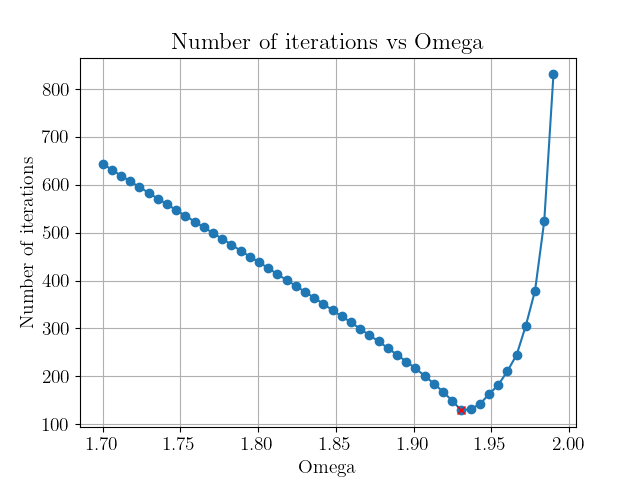
\includegraphics[width=0.7\textwidth]{../fig/lab1/best_omega_122.png}
    \caption{\Shining{Optimal $\omega$ for 4 processors on a 4x1 grid}}
    \label{fig:best_omega_122}
\end{figure}
We find that the optimal $\omega$ is at about $1.93$ for this setup with only 129 iterations. This constitutes a speedup of about 1825\% compared to the sequential implementation. \\

\textbf{N.B.:} If not stated otherwise, we will use $\omega = 1.93$ for the following exercises. 

\subsubsection{Scaling behavior with larger grids}
\label{subsec:scaling}
This investigation is carried out three times: Once with a $4\times 1$ topology (as in the previous section), followed by a $1\times 4$ and a $2\times 2$ topology. We use grid sizes of $200\times 200$, $400\times 400$, $800\times 800$ and $1600\times1600$ and set $\omega = 1.95$ for all runs. All nine simulations are ran using a \texttt{sbatch} script on Delft Blue to change the appropriate input parameters and run the program subseqeuntly (details can be found in the Appendix and online in the \href{https://github.com/etschgi1/HPC}{repository}). The results are shown in \autoref{fig:scaling_123}.

\begin{figure}[H]
    \centering
    \begin{minipage}{0.48\textwidth}
        \centering
        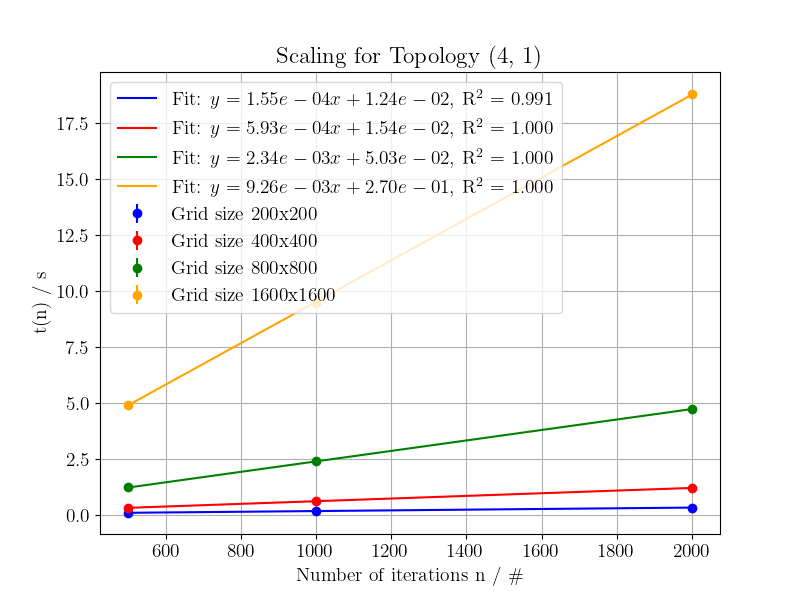
\includegraphics[width=\linewidth]{../fig/lab1/scaling_topology_4x1.png}
    \end{minipage}%
    \hspace{0.02\textwidth}
    \begin{minipage}{0.48\textwidth}
        \centering
        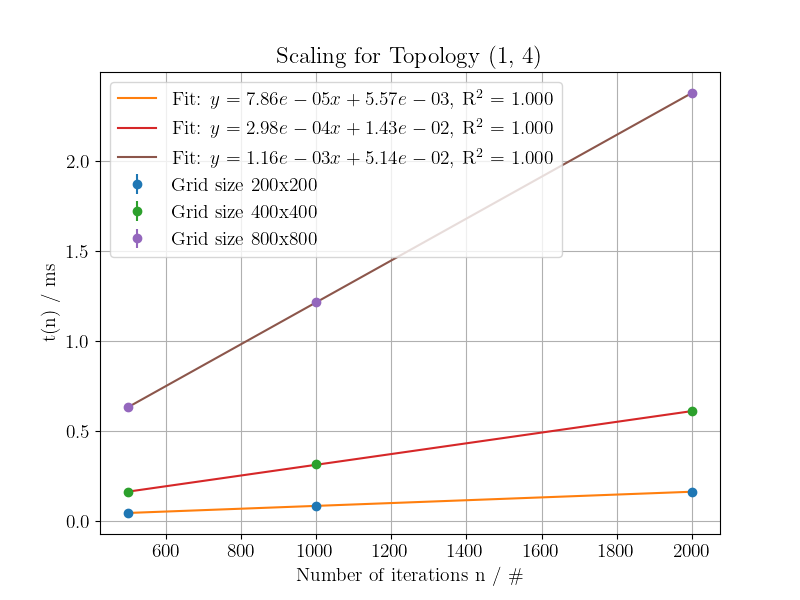
\includegraphics[width=\linewidth]{../fig/lab1/scaling_topology_1x4.png}
    \end{minipage}
    
    \vspace{0.02\textwidth} % Add vertical space between rows

    \begin{minipage}{0.48\textwidth}
        \centering
        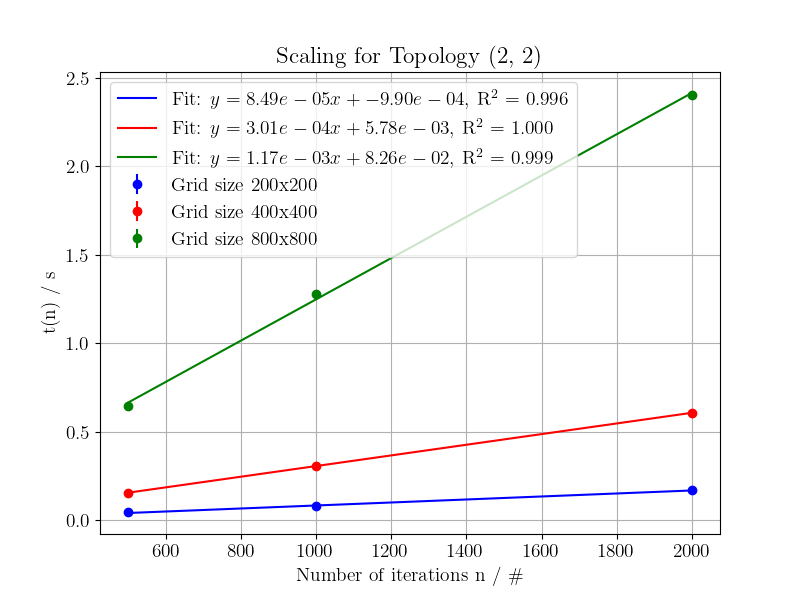
\includegraphics[width=\linewidth]{../fig/lab1/scaling_topology_2x2.png}
    \end{minipage}
    
    \caption{Scaling behavior of the Poisson solver with different grid sizes and processor topologies}
    \label{fig:scaling_123}
\end{figure}

As seen by the high $R^2$ values in the plots, the scaling behavior is very close to linear for the grids. We obtain the following scaling factors for the different grid sizes and topologies from the linear fits:
\begin{table}[H]
    \centering
    \caption{Scaling factors for different processor topologies for the Poisson solver\\Using: $t(n) = \alpha + \beta \cdot n$ as a model}
    \begin{tabular}{|c|c|c|c|}
        \hline
        Topology & Gridsize & $\alpha$ & $\beta$ \\\hline
        $4\times 1$ & $200\times 200$ & $1.24e-02$ & $1.55e-04$ \\ \hline
        $4\times 1$ & $400\times 400$ & $1.54e-02$ & $5.93e-04$ \\ \hline
        $4\times 1$ & $800\times 800$ & $5.03e-02$ & $2.34e-03$ \\ \hline
        $4\times 1$ & $1600\times 1600$ & $2.70e-01$ & $9.26e-03$ \\ \hline
        $1\times 4$ & $200\times 200$ & $3.28e-03$ & $1.61e-04$ \\ \hline
        $1\times 4$ & $400\times 400$ & $7.95e-02$ & $5.86e-04$ \\ \hline
        $1\times 4$ & $800\times 800$ & $5.59e-02$ & $2.41e-03$ \\ \hline
        $1\times 4$ & $1600\times 1600$ & $2.46e-01$ & $9.39e-03$ \\ \hline
        $2\times 2$ & $200\times 200$ & $1.45e-02$ & $1.52e-04$ \\ \hline
        $2\times 2$ & $400\times 400$ & $6.63e-02$ & $5.78e-04$ \\ \hline
        $2\times 2$ & $800\times 800$ & $7.30e-02$ & $2.35e-03$ \\ \hline
        $2\times 2$ & $1600\times 1600$ & $1.79e-01$ & $9.40e-03$ \\ \hline
    \end{tabular}
\end{table}
\Shining{What can you conclude from the scaling behavior?}\\
We see that the scaling behavior is very close to linear for all topologies. This means that the parallel implementation scales as expected with the number of grid points.\\
If we compare the scaling factors ($\beta$) for the topologies we see that the $2\times 2$ topology scales slightly better than the $4\times 1$ and $1\times 4$ topologies (except for the largest grid, where all three topologies scale with a very similar factor). This is not surprising, as the $2\times 2$ topology has a more balanced communication workload balance. In the $2\times 2$ topology every processor has two neighbors, while in the $4\times 1$ and $1\times 4$ topologies the processors at the ends only have one neighbor. This is a general trend: A topology which divides the grid into square / square-like parts will scale better than a topology which divides the grid into long and thin parts.\\
In essence: We want to keep the communication between processors as balanced as possible to achieve the best scaling behavior.\\

\Shining{Scaling of different grid sizes:}\\
We see that larger grids take longer for the same amount of iterations. This is also to be expected, as the number of grid points grows quadratically with the grid size. a $800 \times 800$ grid has 4 times as many grid points as a $400 \times 400$ grid and therefore takes roughly 4 times as long to calculate. 


\subsubsection{Scaling behavior [Theory - no measurements]}
If I could choose between a $16 \times 1$, $8 \times 2$, $4 \times4$, $2 \times 8$, $1 \times 16$ topology, I would choose the $4 \times 4$ topology. This is because the $4 \times 4$ topology has the most balanced communication workload balance, as detailed in the \Shining{Shining} in \autoref{subsec:scaling}.

\subsubsection{Iterations needed for convergence scaling}
We investigate the number of iterations needed for convergence using the $4 \times 1$ topology square grids with sidelength: $10, 25, 50, 100, 200, 400, 800, 1600$. The results for different \Shining{$\omega$} are shown in \autoref{fig:iterations_125}. This test was performed locally as the results are the same for different systems and only depend on the algorithm and the specific problem.

\begin{figure}[H]
    \centering
    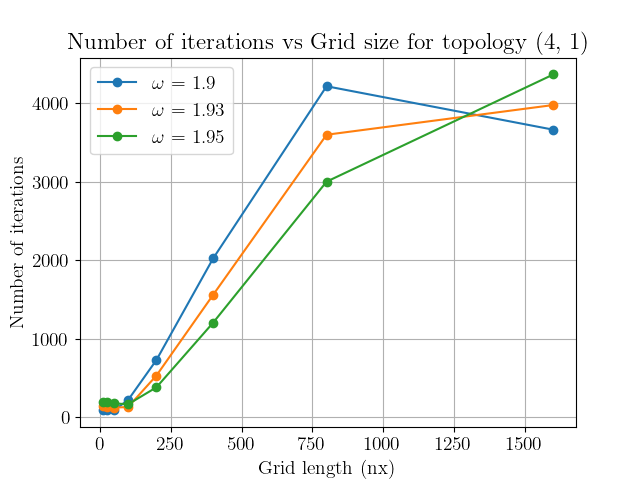
\includegraphics[width=0.7\textwidth]{../fig/lab1/iteration_count_(4, 1)_125.png}
    \caption{Iterations needed for convergence with different grid side lengths}
    \label{fig:iterations_125}
\end{figure}
We can clearly see that the number of iterations till convergence increases with the problem size. At first, I expected linear growth proportional to the number of gridpoints. However, it turns out that the number of iterations actually grow slower and in a square root like fashion. This can be seen by the linear behavior in the plot of grid-side length against iterations. 

\Shining{Why is the number of iterations needed for convergence $\propto \sqrt{g}$?}\\
Our poisson problem is a discretized system in 2D space. The condition number of the matrix we have to solve is proportional to the number of gridpoints in our system. SOR uses the spectral properties of the matrix to solve in a way such that the dominant error mode takes time proportional to the diameter of the domain to converge. This means it is proportional to $\sqrt{g} = \sqrt{n_x \cdot n_y}$.\\

\Shining{Why does omega with the best performance change with the grid size?}\\
As can be seen in \autoref{fig:iterations_125} $\omega = 1.9$ beats the other two values for very small and the largest gridsize. For different gridsizes we get differnetly sized matrices we have to solve. SOR overrelaxes high-frequency errors and underrelaxes low-frequency errors (the later for stability). The optimal $\omega$ is indeed dependent on the gridsize and the error modes present in the system. In our current example, it might be that $\omega = 1.9$ is a good compromise for the grid sizes we are looking at and we are so to say lucky with that specific choice. 

\subsubsection{Error as a function of the iteration number}
With the same $4 \times 1$ topology and grid sizes of $800 \times 800$ the error for $15000$ iterations is tracked using $\omega = 1.93$. The results are shown in \autoref{fig:error_126}.
\begin{figure}[H]
    \centering
    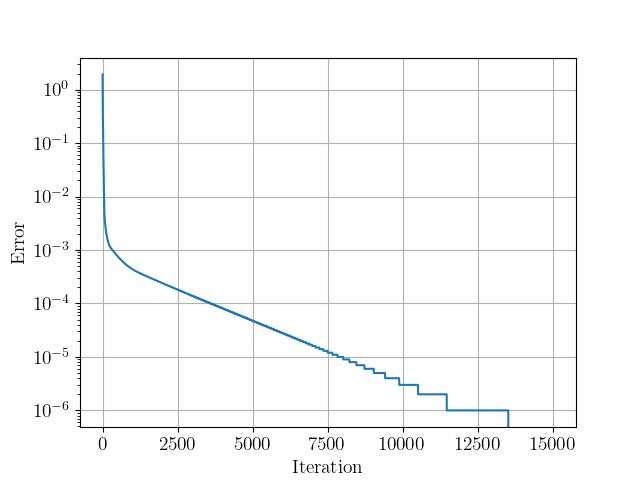
\includegraphics[width=0.7\textwidth]{../fig/lab1/errors_126.png}
    \caption{Error as a function of the iteration number}
    \label{fig:error_126}
\end{figure}
At first the error decreases rapidly in the first few iterations to about $10^{-3}$ (logarithmic scale!). After that the error decreases more slowly until it is below floating point precision.\\ 
\Shining{Note:} All calculations are done using double precision floating point numbers and only the error recording was done using single precision which leaves the step-like artifacts in the plot. Obviously these steps would also be present in the double precision error calculation, but they would be much smaller at comparable iteration numbers and only become visible at much larger iteration numbers. 

\subsubsection{\Shining{Optional} - Gain performance by reducing \texttt{MPI\_Allreduce} calls}
The last subsection showed us that the error reduces monotonically. We might be able to save some time by leaving out some checks and maybe check the global error every 10th or 100th iteration only.\\ First, we should benchmark if it is at all wise to optimize here, by measuring how long the \texttt{MPI\_Allreduce} call takes. We can do this by measuring the time needed for the \texttt{MPI\_Allreduce} call in the \texttt{Do\_Step} function and summing up to get the total time spent in \texttt{MPI\_Allreduce} calls.\\
We again solve with a $4 \times 1$ topology, $\omega = 1.93$ and a $800 \times 800$ grid: It takes roughly $20$ seconds of which the processors spend around 1 - 2 seconds in the \texttt{MPI\_Allreduce} call. This is a significant amount of time: $(7.0 \pm 0.4)$\% of our runtime. This means we would save some time by reducing the number of \texttt{MPI\_Allreduce} calls and calculating 9 (0.25\% of total) more iterations wouldn't hurt us too bad because it takes 3601 to converge!\\
We run the program three times with \texttt{MPI\_Allreduce} calls every 1, 10 and 100 iterations and get the speedups in \texttt{MPI\_Allreduce} calls as shown in \autoref{tab:allreduce_speedup}.
\begin{table}[H]
    \centering
    \caption{Speedup in \texttt{MPI\_Allreduce} calls for different iteration counts and calculated overall speedup (\%)}
    \label{tab:allreduce_speedup}
    \begin{tabular}{|c|c|c|}
        \hline
        Iterations & \texttt{MPI\_Allreduce} - speedup (factor) & calculated overall speedup (\%)\\\hline
        1 (baseline) & 1.00 & /\\\hline
        10 & $6.0 \pm 2.0$ & $ 5.9 \pm 0.5$\\\hline
        100& $62 \pm 6$    & $ 6.9 \pm 0.4$\\\hline
    \end{tabular}
\end{table}
As can be clearly seen from the table we can gain around 6 \% using \texttt{MPI\_Allreduce} calls every 10 iterations and around 7 \% using \texttt{MPI\_Allreduce} calls every 100 iterations. This is a significant speedup for a very small change in the code.\\
\Shining{Note:} The speedup is calculated to account for fluctuations in the runtime of the program, due to other processes running on the same machine / cluster. 

\subsubsection{Reduce border communication}
Another way to reduce communication overhead is to reduce the number of border exchanges. To investigate if this yields a speedup  we run the program on a $4 \times 1$ topology, $\omega = 1.93$ and different grid sizes and track the iterations and time as seen in \autoref{fig:border_speedup}.

\begin{figure}[H]
    \centering
    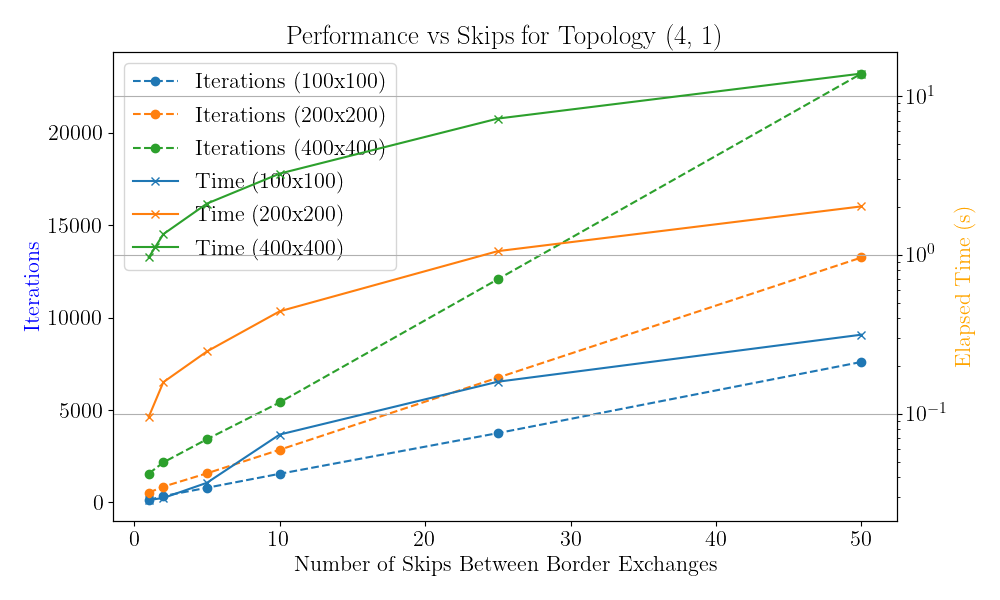
\includegraphics[width=0.7\textwidth]{../fig/lab1/skips_topology_4x1.png}
    \caption{Speedup by reducing border exchanges (4x1 topology)}
    \label{fig:border_speedup}
\end{figure}

Running the with different numbers of skipped border exchanges naturally slows down convergence, meaning we need more iterations to reach the same error. For all tested grid sizes the initial SOR version without skipping border exchanges has the fewest iterations needed to convergence and also the fastes runtime. \\
\Shining{What can you conclude from the results?}\\
We can conclude that reducing the number of border exchanges does not yield a speedup. The reason for this is that we have to calculate more iterations to converge to the solution which outweighs the gains from reduced communication overhead. Interestingly, for the $100 \times 100$ grid there exists a local minimum in time at 4 skipped border exchanges compared to 3 skipped. This is likely due to our source field distribution and thus specific to our problem.\\

Running the problem again with another ($2\times 2$ topology specifically) on our Delft Blue node we get the same qualitative result as seen in \autoref{fig:border_speedup2}. 

\begin{figure}[H]
    \centering
    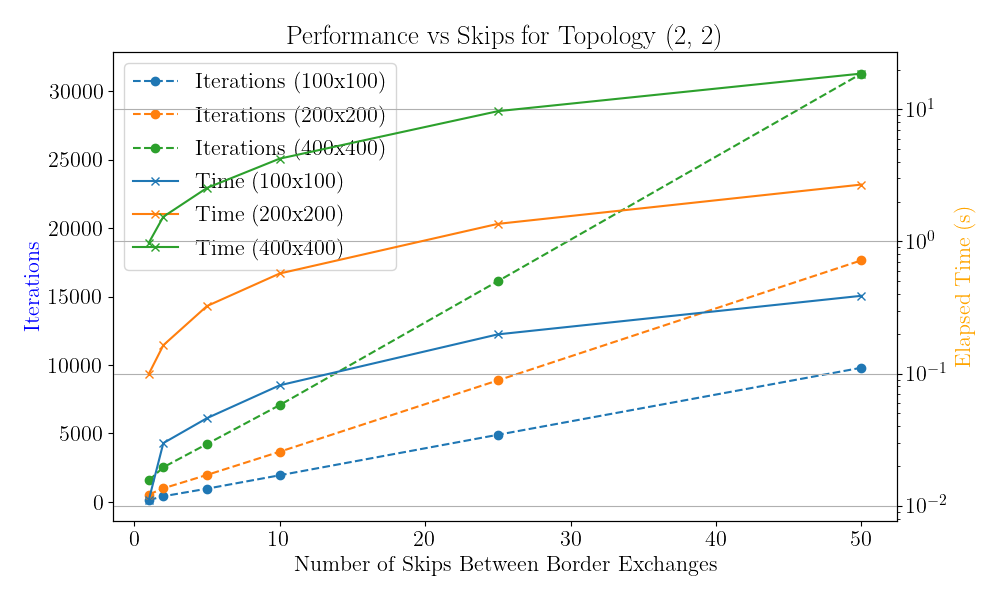
\includegraphics[width=0.7\textwidth]{../fig/lab1/skips_topology_2x2.png}
    \caption{Speedup by reducing border exchanges (2x2 topology)}
    \label{fig:border_speedup2}
\end{figure}
\Shining{Taking a closer look at $2\times 2$ vs. $4\times 1$ topology:}\\
While both have qualitatively the same behavior with the fastest time and lowest iterations recorded for the SOR version without skipping border exchanges, the $2\times 2$ topology has a worse convergence behavior in terms of iterations. This is likely due to the fact that the borders of the local grids for the processors in the $2\times 2$ topology are possitioned in closer proximity to the source coordinates compared to the $4\times 1$ topology. This could explain the observed higher iteration count for convergence in all grid sizes in the $2\times 2$ topology.
\subsubsection{Optimize \texttt{Do\_Step} loop}

In \texttt{Do\_Step} we iterate over the whole grid but only update one of the two parities at a time. This means we can split the loop into two loops, one for each parity. We start out with something like this:
\begin{lstlisting}[language=c]
    for (x = 1; x < dim[X_DIR] - 1; x++){
        for (y = 1; y < dim[Y_DIR] - 1; y++){
            if ((x + offset[X_DIR] + y + offset[Y_DIR]) % 2 == parity && source[x][y] != 1){
                ...
\end{lstlisting}
and we change it to:
\begin{lstlisting}[language=c]
    int start_y;
    for (x = 1; x < dim[X_DIR] - 1; x++){
        start_y = ((1 + x + offset[X_DIR] + offset[Y_DIR]) % 2 == parity) ? 1 : 2;
        for (y = start_y; y < dim[Y_DIR] - 1; y += 2){
            if (source[x][y] != 1){
                ...
\end{lstlisting}
The basic idea is to avoid y-coordinates which are not in the parity we are currently updating. 
We measure 10 runs for a $800 \times 800$ grid and a $4 \times 1$ topology with $\omega = 1.93$ and get the following times: 
\[t_{\text{no\_improvements}} = \SI{5.59(5)}{\second}\hspace{1cm}\text{and}\hspace{1cm}t_{\text{loop\_improvements}} = \SI{4.64(7)}{\second}\]
So we get a minimal speedup of about 17\% by optimizing the loop which is a enormous speedup for such a small change.

\Shining{Why does this make such a difference}\\
The reason for this is that we avoid unnecessary looping and if statements. This means that we have less overhead in the loop and can therefore calculate faster by skipping the unnecessary loop entries. 

\subsubsection{\Shining{Optional} - Time spent within \texttt{Exchange\_Borders}}
We can measure the time spent in \texttt{Exchange\_Borders} by adding a timer to the function. We run the program with $\omega = 1.93$ and different topologies\footnote{\{(2,2), (3,3), (4,4), (5,5), (6,6), (2,3), (2,4), (2,5), (3,4)\}} and grid sizes and get the results shown in \autoref{fig:exchange_time}.
\begin{figure}[H]
    \centering
    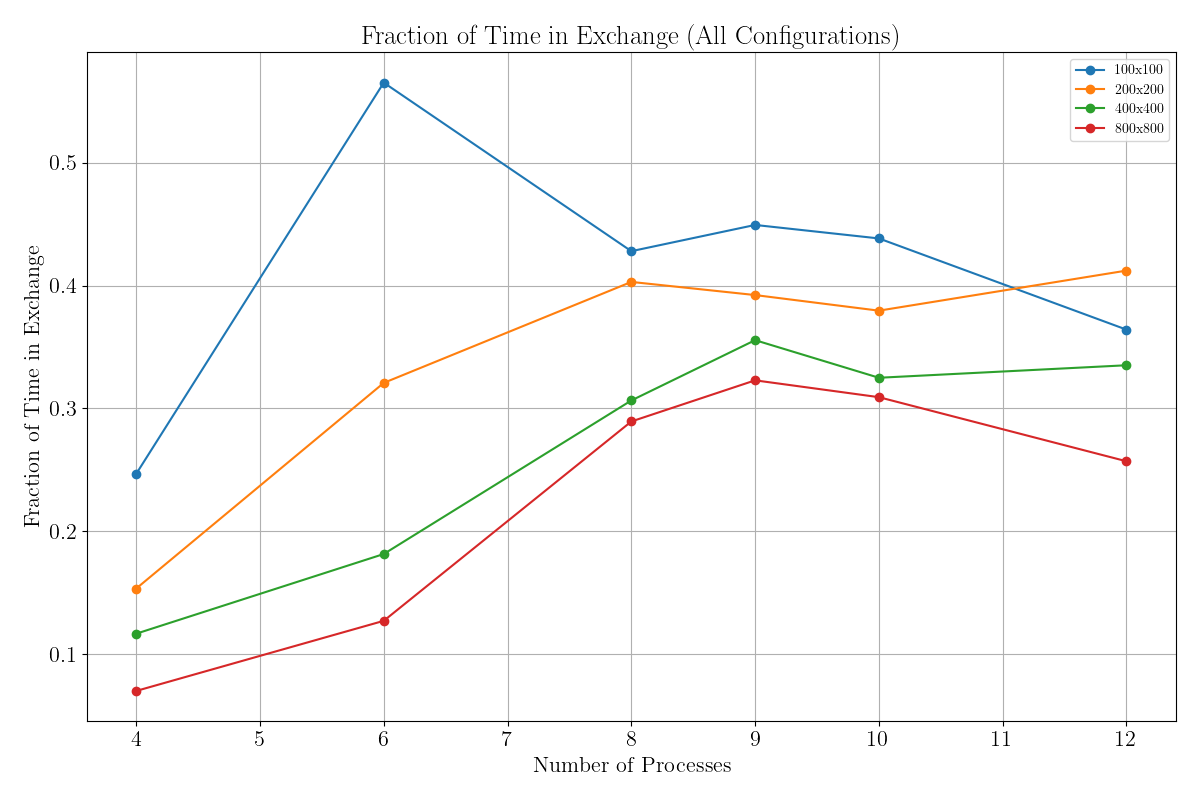
\includegraphics[width=0.85\textwidth]{../fig/lab1/fraction_exchange_comparison_connected.png}
    \caption{Fraction of total time spent in \texttt{Exchange\_Borders}}
    \label{fig:exchange_time}
\end{figure}
As we can clearly see, the time spent in \texttt{Exchange\_Borders} is initially smaller and grows with processor count with some remarkable peaks especially for small grids and certain processor topologies. The curves are generally shifted downward for larger gridsizes. \\

\Shining{Interpretation:}\\
One would expect larger grid sizes to be more computationally expensive and we have already established that iterations take longer the bigger the grid. Communication obviously also takes longer for a larger grid because we have more data to sent. However, the circumference of a square grows linearly, while the area grows quadratically. The quadratic growth of the area is the reason for the downward shift in the curves for larger grid sizes because the communication overhead grows slower than the computational overhead for larger grids.\\
Besides the peaks at $p=6$ and $p=12$ we see a general trend of increasing time spent in \texttt{Exchange\_Borders} increasing processor count. This is not surprising as we have more processes which have to communicate with each other and the data locality is worse for larger processor counts.

\Shining{When is the time spent in \texttt{Exchange\_Borders} significant / comparable to computation?}\\
As can be seen in \autoref{fig:exchange_time} the time spent in \texttt{Exchange\_Borders} is significant for all grid sizes from the start (between 2.5 and 7.5\%). Thereafter it peaks for $p=6$ and again for $p=12$ to around 5\% to 38\% and 10\% to 54\% respectively. This means that the time spent in \texttt{Exchange\_Borders} is significant for all grid sizes and processor counts, but especially as the processor count grows.

\subsubsection{Latency and bandwith in \texttt{Exchange\_Borders}}
We use the configurations from \autoref{subsec:scaling}: $4 \times 1$, $2 \times 2$ and \Shining{$3 \times 3$} topologies with grid sizes of $200 \times 200$, $400 \times 400$ and $800 \times 800$ and $\omega = 1.95$ as well as the other settings set to their defaults. We obtain the results in \autoref{tab:latency_bandwith}.
\begin{table}[H]
    \centering
    \caption{Metrics for \texttt{Exchange\_Borders} latency and bandwith}
    \label{tab:latency_bandwith}
    \begin{tabular}{|c|c|S[table-format=3.1(2.1)]|S[table-format=2.1]|S[table-format=10]|S[table-format=8]|}
    \hline
    Topology & Grid Size & {Latency (ms)} & {Latency (\%)} & {Bandwidth (\si{\byte\per\second})} & {Total Data (\si{\byte})} \\\hline
    4x1 & 200x200 & 2.0(0.6)& 3.9  & 2034737840 & 3104896 \\\hline
    4x1 & 400x400 & 9.8(4)  & 1.4  & 2005275269 & 19450368 \\\hline
    4x1 & 800x800 & 51(23)  & 0.8  & 2112229431 & 96480384 \\\hline
    2x2 & 200x200 & 3.6(1.0)& 5.0  & 541474183  & 2493696 \\\hline
    2x2 & 400x400 & 17(7)   & 2.3  & 668287123  & 15591168 \\\hline
    2x2 & 800x800 & 92(37)  & 1.4  & 665489803  & 77261184 \\\hline
    3x3 & 200x200 & 161(80) & 43.9 & 9006796    & 1686912 \\\hline
    3x3 & 400x400 & 105(53) & 18.9 & 56268947   & 10419840 \\\hline
    3x3 & 800x800 & 219(67) & 6.2  & 2369103880 & 51603552 \\\hline
    \end{tabular}
\end{table}
\Shining{Interpretation:}\\
As can be seen the latency is lowest for the $4\times1$ topology followed by $2\times2$ and $3\times3$. This is not surprising as the $4\times1$ topology has the least amount of neighbors to communicate with per processor. The worst latencies can generally be observed for the $3\times3$ topology because every processor has to communicate with 2,3 or 8 neighbors. As can be seen by the huge discrepancy in the latency percentage for the $3\times3$ topology, the latency is strongly dependent on the grid size (problem size). While nearly half of the time is spent in latency for the $200 \times 200$ grid, only 6.2\% of the time is spent in latency for the $800 \times 800$ grid.\\

\subsubsection{Exchange Border potential improvements}
Indeed we communicate twice as much as we need after each \texttt{Do\_Step} call. We shall analyze this considering the following points: 
\begin{itemize}
    \item address of the first point to exchange: This depends on the parity of the processor. It is simply the first or second point in the grid depending on the parity (leaving out the edge case where the processor only has one data-point).
    \item the number of points to exchange: This normally is the number of points in the grid minus ghost cells divided by two. However, this may change if there is an odd number of points in the grid (then we have to exchange one more or one less point).
    \item the number of points in between grid points that have to be exchanged: The stride of the data will change. Currently we exchange every point for one direction and every \texttt{dim[Y\_DIR]}-th point for the other direction. This can be optimized to exchange every second point in one direction and every second \texttt{dim[Y\_DIR]}-th point in the other direction. 
\end{itemize}

\textbf{Is it worth it?}\\
For smaller gridsizes it is not worth it to optimize the border exchange. The time spent in the border exchange might be significant in relative terms, but the absolute time is still small. For larger gridsizes it might be worth it to optimize the border exchange. As we have seen, this becomes more significant as the processor count and gridsizes grow. For our current problem and similarly sized problems the effort put into optimizing the border exchange is certainly not worth it.
\newpage


\section{Finite elements simulation}
\label{sec:fempois}
We will now shift our focus to a more general grid which is based on triangulation. In this section we will compare our parallel implementation from the previous section and disect the differences and similarities. For that reason we shall use the same sources in our grid as given in \texttt{sources.dat}. \\
Note that the sections for the exercises will be labeled as (2.1, 2.2, 2.3, ...) corresponding to exercises (4.1, 4.2, 4.3, ...) in the lab manual.\\
\subsection{Code understanding \& \texttt{Exchange\_Borders}}
The first step is to read through the code in \textbf{MPI\_Fempois.c} and to understand it. Furthermore, we have to implement the \texttt{Exchange\_Borders} function for which only a skeleton is given. The function should exchange the border values of the local grid with the neighboring processes.\\ 
The implementation of this function is quite straight forward. We only have to loop over all the neighbors of a process and send out the border values and receive the border values from the neighbors. The function is implemented as follows:

\begin{lstlisting}[language=c]
void Exchange_Borders(double *vect)
{
    for (size_t i = 0; i < N_neighb; ++i)
    {
        MPI_Sendrecv(vect, 1, send_type[i], proc_neighb[i], 0, //send
                     vect, 1, recv_type[i], proc_neighb[i], 0, //recv
                     grid_comm, &status);
    }
}
\end{lstlisting}

\subsection{Time benchmarking}
\label{subsec:timing_fe}
Next we turn our attention to timing of different sections in the code. \\
We have to measure: 
\begin{itemize}
    \item Time spent in computation 
    \item Time spent exchanging information with neighbors
    \item Time spent doing global communication
    \item Idle time
\end{itemize}
We setup the following variable to measure / deduce the time spent in the different sections:
\begin{lstlisting}[language=c]
    double total_time = 0.0;
    double exchange_time_neighbors = 0.0;
    double exchange_time_global = 0.0;
    double compute_time = 0.0;
\end{lstlisting}

We will measure the time spent in computations by timing the solve function and subtracting the time spent in the \texttt{MPI\_Allreduce} calls. The time spent in the \texttt{MPI\_Allreduce} calls is the time spent in global communication. The time spent in exchanging information with neighbors is the time spent in the \texttt{Exchange\_Borders} function. Finally, the idle time can be determined by summing up the differences between the cores total time and the slowest cores total time. \underline{Note} that this way of calculating the idle time is an approximation since it is assumed that the slowest core doesn't have any idle time. However, I've discussed this with the TA and he said that this is a valid way of calculating the idle time for this exercise.\\
The commandline output for runs is as shown in \autoref{fig:timing2} for an example run: 
\begin{figure}[H]
    \centering
    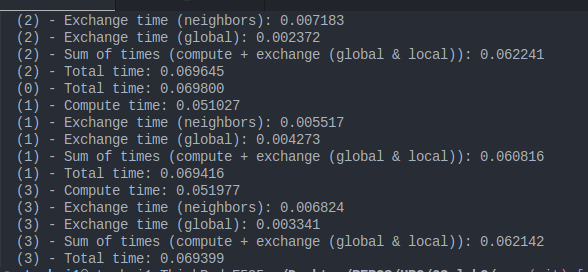
\includegraphics[width=0.7\textwidth]{../fig/lab2/ex2.png}
    \caption{Timing for the different sections.\\
    (x) \dots denotes the process rank\\
    Compute time \dots time spent in the \texttt{solve} function \underline{only on computing}\\
    Exchange time (neighbors) \dots time spent in \texttt{Exchange\_Borders} \\
    Exchange time (neighbors) \dots time spent in \texttt{MPI\_Allreduce} calls \\
    Sum of times \dots total time spent in compute and communication (excluding setup / idle time)\\
    Total time \dots total time spent in the program\\
    }
    \label{fig:timing2}
\end{figure}

The \underline{idle time} is calculated as denoted above and therefore not shown in the output in \autoref{fig:timing2}. We get the following results from our Delft Blue runs in \autoref{tab:timing}:


\begin{table}[H]
    \centering
    \caption{Rank averaged time benchmark for different grid sizes and topologies.\\ All \underline{times are in milliseconds (ms)}.\\\textbf{Note:} WTime does also include setup and teardown (mallocs, frees, etc.) - therefore the sum of the times is not equal to WTime.}
    \label{tab:timing}
    \begin{tabular}{|l|l|S[table-format=4.1]|S[table-format=4.1]|S[table-format=2.1]|S[table-format=2.1]|S[table-format=2.1]|}
        \hline
        Top. & {{{Grid Size}}} & {{{WTime (avg)}}} & {{{Comp. (avg)}}} & {{{Ex. Neighb. (avg)}}} & {{{Ex. Global (avg)}}} & {{{Idle (avg)}}} \\\hline
        1x4 & 100x100 & 82.0 & 18.6 & 1.3 & 1.7 & 9.0 \\\hline
        1x4 & 200x200 & 194.5 & 150.6 & 3.6 & 6.8 & 12.1 \\\hline
        1x4 & 400x400 & 1498.2 & 1357.8 & 10.1 & 26.4 & 9.1 \\\hline
        2x2 & 100x100 & 43.7 & 18.6 & 1.6 & 1.4 & 9.1 \\\hline
        2x2 & 200x200 & 184.0 & 145.2 & 4.3 & 8.1 & 5.7 \\\hline
        2x2 & 400x400 & 1428.7 & 1279.2 & 11.5 & 22.4 & 25.6 \\\hline
    \end{tabular}
\end{table}
We see that the total time is comparable between the two topologies for all grid sizes. Furthermore, the total runtime also increases non-surprisingly with the gridsize. \\

\Shining{Why does computation time increase faster than linearly?}\\
One could expect, that the grid with $200\times200$ elements would take 4 times as long as the grid with $100\times100$ elements. However, the runtime roughly 8 times longer. This happens because additionally to the higher number of grid points the algorithm also takes longer (more iterations) to converge and hence the computation time is longer. \\

\Shining{Analysis of the different times}\\
To get a better grasp on the data a stacked bar plot, as shown in \autoref{fig:timingbar}, is created. We immediately see that the bulk of the time is spent on computing the solution. The second biggest contributor is the global exchange time and the idle time, followed by local exchange time.\\
That computation takes up the biggest part of the time is of non surprise especially on the bigger grids this is to be expected. Rather surprisingly the global excahnge time takes up a lot of time. This begs the question why two lines of the form:
\begin{lstlisting}[language=c]
MPI_Allreduce(... , ... , 1, MPI_DOUBLE, MPI_SUM, grid_comm);
\end{lstlisting}
take up this much time. This actually comes down to masked idle time. While the operation itself only sums up the values of 4 double, the operation is blocking and therefore the other cores have to wait for the slowest core to finish. If we look back at the definition of idle time, we defined it as the difference of the total time of the slowest core and the total time of the current core. However, as stated above, this does not take waiting time in MPI calls (like \texttt{MPI\_Allreduce}) into account. Certainly, this explains now that the global exchange time is high, because every core has to wait for the others to synchronize to compute the \texttt{MPI\_Allreduce}.\\
\begin{figure}[H]
    \centering
    \begin{minipage}{0.48\textwidth}
        \centering
        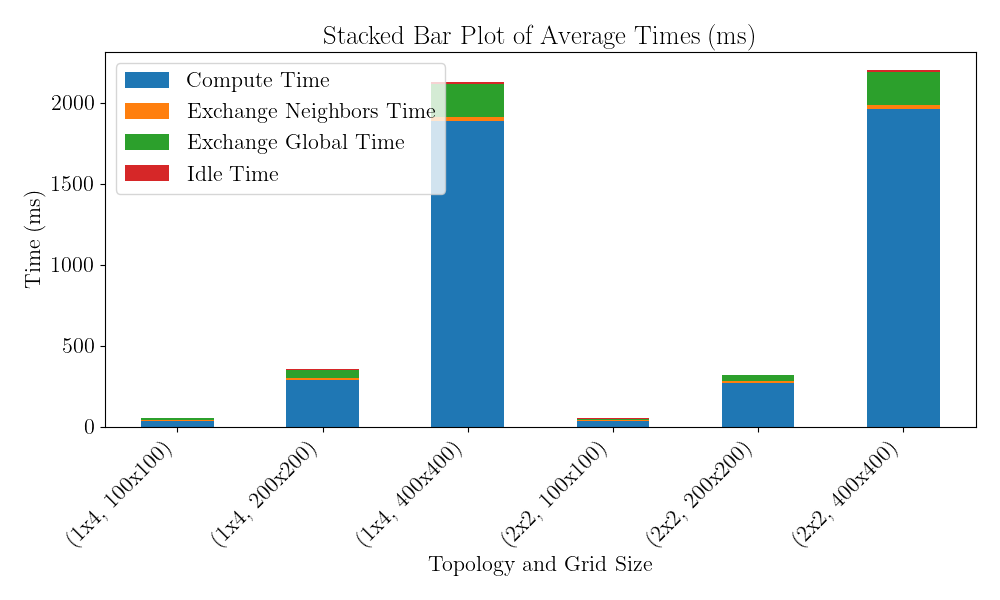
\includegraphics[width=\linewidth]{../fig/lab2/average_times_stacked_bar_22.png}
    \end{minipage}%
    \hspace{0.02\textwidth}
    \begin{minipage}{0.48\textwidth}
        \centering
        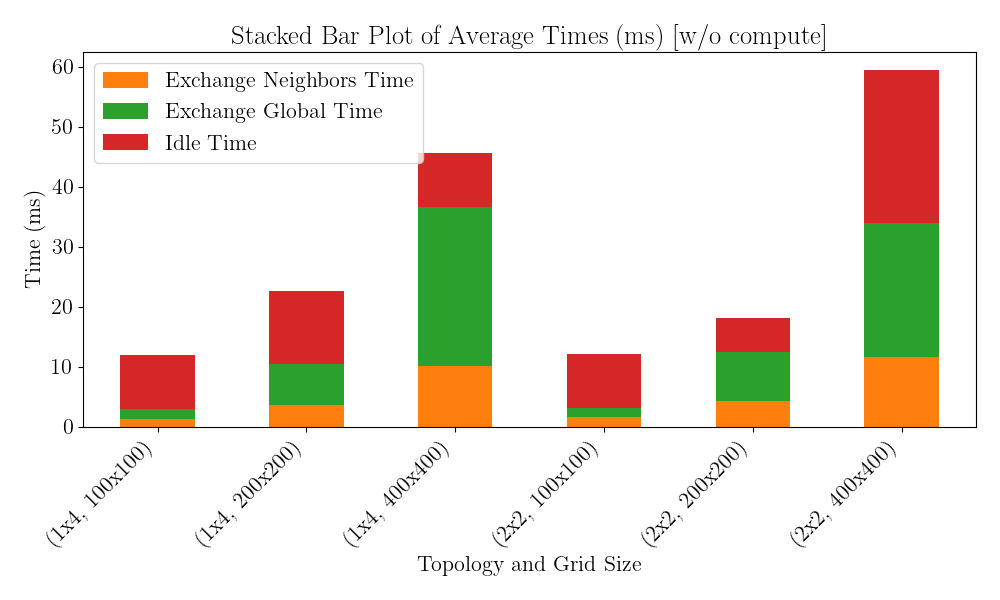
\includegraphics[width=\linewidth]{../fig/lab2/average_times_stacked_bar_no_comp_22.png}
    \end{minipage}
    \caption{Scaling behavior of the Poisson solver with different grid sizes and processor topologies.\\
    with compute time (left) and without compute time (right).}
    \label{fig:timingbar}
\end{figure}
We conclude that most of the time spent on communication in our solver is actually due to the waiting time in the \texttt{MPI\_Allreduce} calls and the other idle time (waiting for the slowest core to finish). The actual exchange of data only represents a fraction of this time. Biggest, especially for larger grids, contributor for the time is still the computation which takes up north of 95\% of the total time on larger grids.\\
\subsection{Data exchange amount}
This section is about the amount of data exchanged each iteration among one process with all its neighbors.\\
We assume a uniformly triangulated grid which is partitioned stripe-wise and distribution over $P$ processes. Furthermore, we assume that each process has to send the same amount of data. Indeed, this is not generally the case but for examples with periodic boundary conditions this is for example a valid assumption.\\
Now we see that every process has to communicate with $2d$ neighbors, where $d$ is the dimension of the grid, under our assumptions there are $2$ neighboring processes. With the assumption of a $n^2$ grid, our process communicates $n$ values with each of these neighbors. For striped partitioning we get: 
\begin{equation*}
    \text{Data exchanged per Process} = 2n 
\end{equation*}
or in total: 
\begin{equation*}
    \text{Data exchanged} = 2n \cdot P 
\end{equation*}
Let's check for the extreme case $1000\times1000$ grid and $P=500$ processes. We get:
\begin{equation*}
    \text{Data exchanged} = 2\cdot1000\cdot500 = 1000000
\end{equation*}
Which is the same amount of data as there are datapoints. This makes sense because every process has to communicate the top row upwards and the bottom row downwards.\\
Note, that we could even do worse if we assigned every process a single row. In this case every process would have to communicate the same data upward and downward. This would result in a data exchange of $2\cdot1000\cdot1000 = 2000000$ which is double the amount of data as there are datapoints.\\
For a box partitioning a process has to communicate $\nicefrac{n}{\sqrt{P}}$ (assuming divisibility with all neighbors) with each of its 4 neighbors. We get:
\begin{equation*}
    \text{Data exchanged per Process} = 4 \cdot \nicefrac{n}{\sqrt{P}}
\end{equation*}
or in total: 
\begin{equation*}
    \text{Data exchanged} = 4 \cdot n \cdot \sqrt{P}
\end{equation*}
This means that a striped partitioning is less efficient compared to a boxed partitioning starting from $P=4$, as can be seen in \autoref{fig:dataexchange}.\\
\begin{figure}[H]
    \centering
    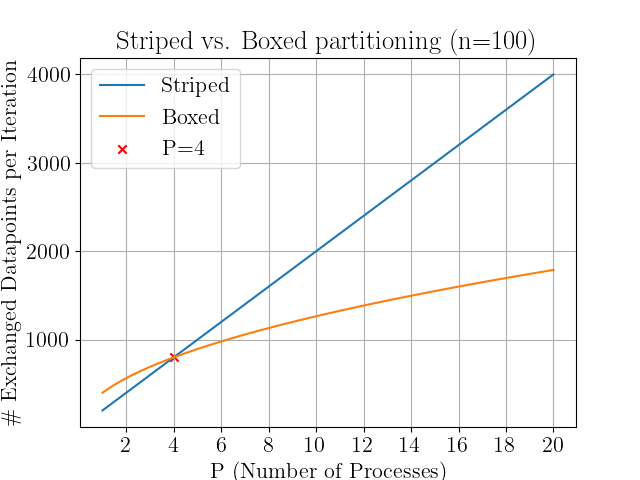
\includegraphics[width=0.5\textwidth]{../fig/lab2/scale23.png}
    \caption{Striped vs. Boxed partitioning on a $100\times100$ grid using $P$ processors.}
    \label{fig:dataexchange}
\end{figure}
\subsection{Unbalanced communication}
In the last section we assumed that every process has to communicate with the same amount of neighbors in our given scenario. That is actually not entierly true. There is an imbalance, even if just a small one.\\ 

\Shining{But where does this imbalance come from?}\\
Let's take a look at a \Shining{uniformly triangulated grid} with $P=4$ processes. We assume that the grid is box-partitioned as given in \autoref{fig:boxpart24}.\\
\begin{figure}[H]
    \centering
    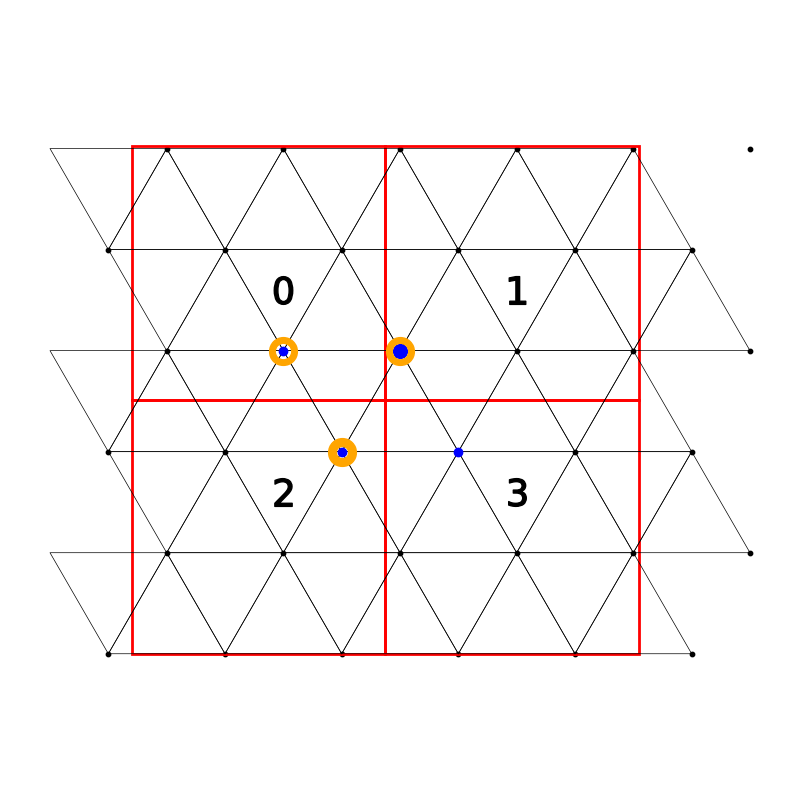
\includegraphics[width=0.5\textwidth]{../fig/lab2/grid24.png}
    \caption{Box partitioning of a uniformly triangulated grid with $P=4$ processes.\\
    One point (big-blue) in $1$ (and similarly in $3$) has to communicate its value to 3 neighbors (small-blue).\\
    Another point (big-orange circle) in $2$ (and similarly in $4$) has to communicate its value to 2 neighbors (small-orange circles).}
    \label{fig:boxpart24}
\end{figure}
We see that the geometry of a given uniform triangulated grid leads to an imbalance in communication. This imbalance is usually not a big problem, especially for bigger grids with comparably small amounts of processors because only 2 points have to communicate with 3 neighbors. However, for smaller grids or proportionally high processor counts the imbalance is more significant.\\ 

Looking at a $3\times3$ grid with $P=9$ processors, we see that the imbalance is more significant as shown in \autoref{fig:boxpart243}.\\
\begin{figure}[H]
    \centering
    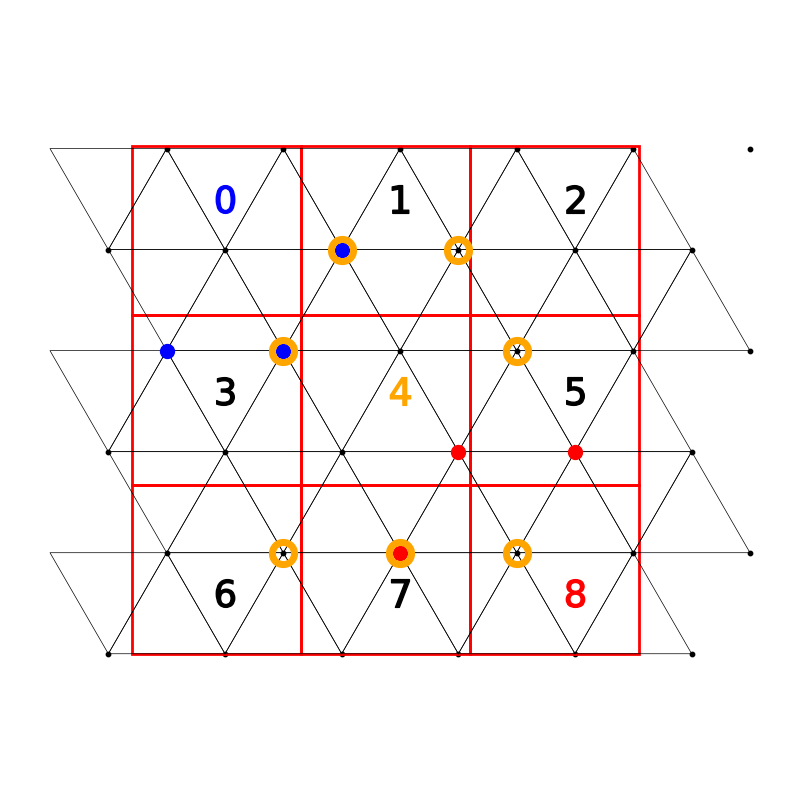
\includegraphics[width=0.5\textwidth]{../fig/lab2/grid_3x3_partition.png}
    \caption{Box partitioning of a uniformly triangulated grid with $P=9$ processes.\\
    Corner (0/8 - blue/red) processes have to communicate their values to 2 or 3 neighbors respectively (1 and 3 - blue or 4, 5 and 7 - red).\\
    Central (4 - orange) processes have to communicate their value to 6 neighbors (1, 3, 5, 6, 7 and 8).}
    \label{fig:boxpart243}
\end{figure}
As we can see the imbalance comes from the partitioning geometry on the uniform triangulated grid. Because our processor grid is rectangular the results will always, in one way or another come out as shown in the schematic above.\\
For $3\times3$ grid we have 4 corner processes which have to communicate with 2 or 3 neighbors and 1 central process which has to communicate with 6 neighbors. This is a significant imbalance and compared to the $2\times2$ grid it is not negligible, because the central process has to communicate more than 2 extra points (whole edges of datapoints) to its neighbors.\\
\subsection{Estimates for computation $\equiv$ communication time}
\Shining{N.B.} This section will use two different ways to estimate the equilibrium point.\\

1) Let's assume that we have 4 processes and want to estimate for which grid size the computation time is equal to the communication time. 
One way to estimate this is by fitting a polynomial of degree 2 to the computation and a linear fit to the exchange time for our measurements in \autoref{tab:timing} and find the point where the times are equal. Thereafter we can use this information to determine the grid size where this happens. This process gives us a \underline{value of $n\approx84$} for the grid size as shown in \autoref{fig:comp_eq_comm}\\

\begin{figure}[H]
    \centering
    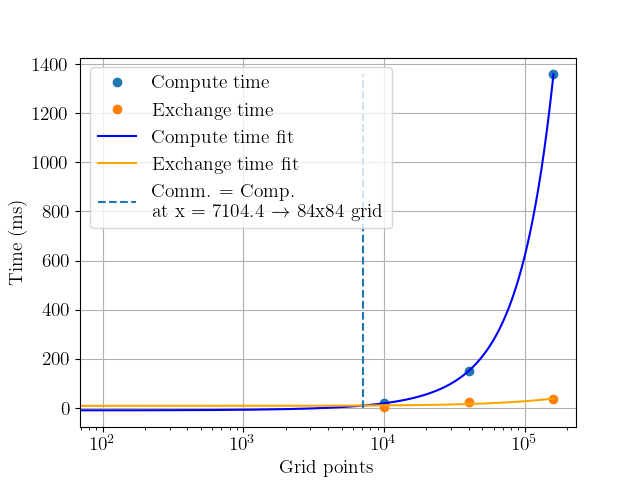
\includegraphics[width=0.5\textwidth]{../fig/lab2/estimate25.png}
    \caption{Fitting expected computation time $\equiv$ communication time for 4 processes.}
    \label{fig:comp_eq_comm}
\end{figure}

2) We'll also estimate this equilibrium point for a $1000\times1000$ grid. However, this time around we'll actually use a different way of calculating the number of Processes. We use the definitions from the lecture for stencil type computation: 
\begin{itemize}
    \item Computation time: $T_{\text{S}} = \text{number\_ops} \cdot t_\text{op} \sim  4 t_\text{op} \cdot n^2 \hspace{5mm} \text{(for stencil type - overall)}$
    \item Communication time: $T_{\text{comm}} = \text{number\_comm} \cdot t_\text{comm} \sim 2 n \cdot t_\text{data}\hspace{5mm} \text{(for stencil type - overall)}$
\end{itemize}
Note that the definitions above \underline{apply for a single iteration and \textbf{one} processor!}\\
We can calculate the time for communication from the data in \autoref{tab:timing} as follows: 
\[t_\text{data}(P) = \frac{t_\text{global\_comm}+t_\text{neighbor\_comm}}{2\cdot n \cdot P \cdot \#_\text{{iterations}}}\]
Similarly we can calculate the time for computation as follows:
\[t_\text{op} = \frac{t_\text{comp.}}{4 \cdot n^2 \cdot \#_\text{{iterations}}}\]
Note that the later doesn't depend on the number of processes.\\
Using the data from \autoref{tab:timing} we determine that one operation takes $t_\text{op} = \SI{3.3(3)e-6}{\milli\second}$. From that we can determine the computation time $t_{\text{comp.}}$ for $n=1000$ as follows:
\[t_{\text{comp.}} = 4 \cdot n^2 \cdot t_\text{op} \cdot \#_\text{{iterations}} = 4 \cdot 1000^2 \cdot 3.3(3) \cdot 10^{-6} \cdot 1241 = \SI{17.8(15)}{\second}\]
where 1241 ($\#_\text{{iterations}}$) is the number of iterations to converge. We set $t_{\text{comp.}} = t_{\text{data}}$ and solve for $P$. We need values for $t_\text{global\_comm}$ and $t_\text{neighbor\_comm}$ and take a look at \autoref{fig:comp_eq_comm} and decide to further investigate the trend for the excahnge time ($= t_\text{global\_comm} + t_\text{neighbor\_comm}$). We decide to use a linear extrapolation as shown in \autoref{fig:comp_sencil_extra}. We get an estimated communication time of $\SI{100}{\milli\second}$. \\

Now we have everything to solve for P and using 1241 for $\#_\text{{iterations}}$ again we get $P = \num{29(3)}$ processes. 
\begin{figure}[H]
    \centering
    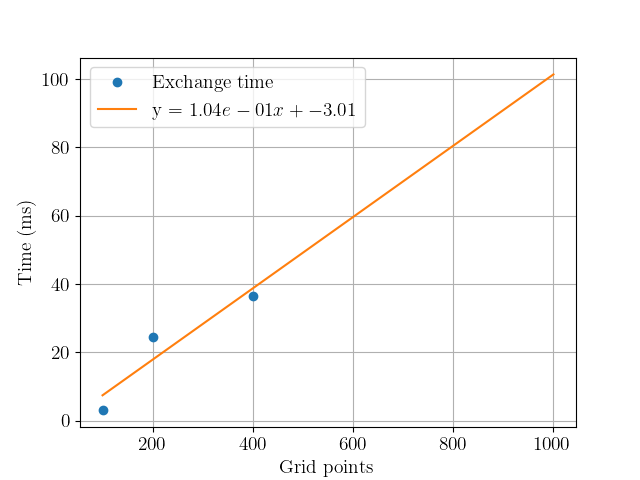
\includegraphics[width=0.5\textwidth]{../fig/lab2/estimate25_stencil.png}
    \caption{Extrapolating the communication time for $n=1000$ using a linear fit.}
    \label{fig:comp_sencil_extra}
\end{figure}

Our predictions are: a $84\times84$ grid for 4 processes with equal computation and communication times and a $1000\times1000$ grid for 29 processes (also having equal computation and communication time).\\
We measure the ratio \nicefrac{$t_{\text{comp}}$}{$t_{\text{comm}}$} and get the following results for a $4\times1$ topology in \autoref{tab:comp_comm_ratio}:

\begin{table}[H]
    \centering
    \caption{Ratio of computation to communication time for different grid sizes.}
    \label{tab:comp_comm_ratio}
    \begin{tabular}{|c|S[table-format=1.2(1.2)]|}
        \hline
        {{{Grid Size}}} & {Ratio} \\\hline
        10x10 & \num{0.53(0.06)} \\\hline
        20x20 & \num{0.84(0.15)} \\\hline
        30x30 & \num{0.86(0.13)} \\\hline
        40x40 & \num{1.97(0.24)} \\\hline
        50x50 & \num{2.66(0.61)} \\\hline
        75x75 & \num{4.37(1.00)} \\\hline
        84x84 & \num{3.70(0.85)} \\\hline
        90x90 & \num{6.06(1.94)} \\\hline
    \end{tabular}
\end{table}
We see that our initial guess of $84\times84$ grid for 4 processes is off by a long-shot. However, we also notice that the ratio is highly volatile as can be seen by the high uncertainties on the ratio.\\\underline{A rerun of the code produced notably different ratios (e.g. $\num{1.35(25)}$ for $30\times30$ grid)}. It seems that the actual position of the equilibrium point is around $n=35$. Being a physicis, I have to say that our initial guess was of the same magnitude and therefore actually not too far off by our standards \smiley.\\

Let's see how our prediction for the $1000\times1000$ grid with 29 processes holds up. Using a $29\times1$ topology we get $\num{4.04(1.83)}$ for the ratio. It seems we have made a lower prediction in terms of $P$ for the equilibrium point. However, the ratio is in the same ballpark as the ratio for the $84\times84$ grid which is not surprising since we used the same underlying data to make the prediction.\\
\subsection{Adaptive gird}
We will now make our grid denser in the source point areas. \texttt{GridDist} already implements an argument (\textit{adapt}) for that purpose. In order to gauge the speed of convergence we let process 0 print the current precision of the solution. We perform runs with a reference and a denser grid to compare the convergence speed, convergence count and amount of computing time for a $2\times2$ topology and a $100\times100$, $200\times200$ and $400\times400$ grids.\\
We first take a look at the iterations needed for convergence using the standard percision goal of $0.0001$ we get the results in \autoref{tab:adapt_it_count}.\\
It becomes clear that the adaptive grid needs a few more iterations to converge. This is most likely due to the fact that the dense region near the sources initially lead to a slower \glq spreading\grq\, of the solution near the source.\\
\begin{table}[H]
    \centering
    \caption{Iterations needed for convergence on $2\times2$ topology for different grid sizes with and without adapt keyword.}
    \label{tab:adapt_it_count}
    \begin{tabular}{|c|c|c|c|}
        \hline
        {{{Grid Size}}} & {100x100} & {200x200} & {400x400} \\\hline
        {Iterations Reference} & 141 & 274 & 529 \\\hline
        {Iterations Adapt} &     146 & 278 & 532 \\\hline
    \end{tabular}
\end{table}
\Shining{Does such a distored grid lead to faster convergence?}\\
We can answer this questin with a clear no, at least in terms of iterations. Next we'll look at the time it takes to converge.\\

A bar-plot of the time till convergence is shown in \autoref{fig:adapt_time}. We see that the time till convergence is roughly the same for the reference and the adaptive grid. This is not surprising since the time till convergence is mainly determined by the number of iterations needed. 

\begin{figure}[H]
    \centering
    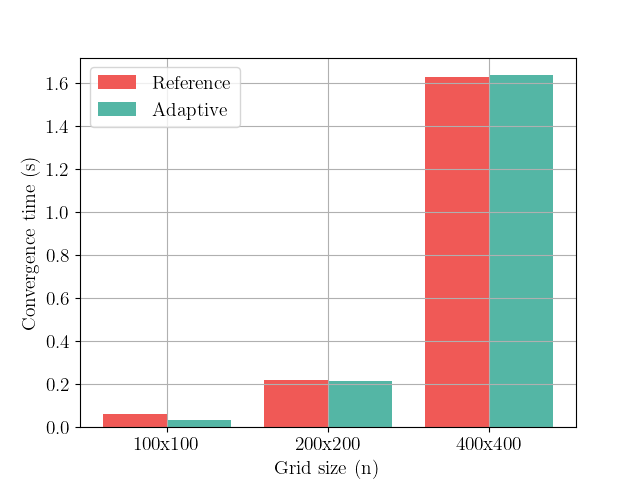
\includegraphics[width=0.5\textwidth]{../fig/lab2/adapt_time.png}
    \caption{Time till convergence (with setup) on $2\times2$ topology for different grid sizes with and without adapt keyword.}
    \label{fig:adapt_time}
\end{figure}
\Shining{Does it affect the speed of convergence?}\\
Also no for this one. The time for the reference / adaptive grid is roughly the same with one exception for the $100\times100$ grid.\\
\begin{figure}[H]
    \centering
    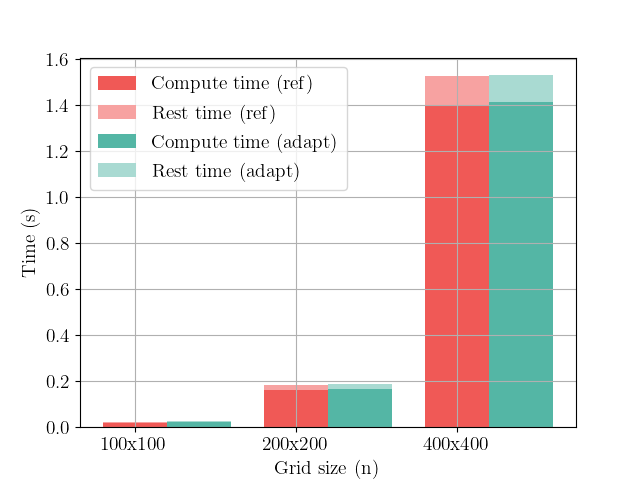
\includegraphics[width=0.5\textwidth]{../fig/lab2/adapt_stacked_time.png}
    \caption{Time till convergence (without setup) on $2\times2$ topology for different grid sizes with and without adapt keyword.}
    \label{fig:adapt_time2}
\end{figure}
If we stack the time needed for computation and communication we see that the computation as well as the communication time is roughly the same for the reference and the adaptive grid as shown in \autoref{fig:adapt_time2}.\\

\Shining{Does it affect the amount of computing time?}\\
So again no, the amount of computing time is roughly the same for the reference and the adaptive grid.\\

\Shining{Why is there hardly any difference between the two?}\\
It seems that in our rather simple example (3 sources) the adaptive grid doesn't lead to a faster convergence. This can likely be attributed to the low complexity of our problem. Due to this low complexity our convergence in iterations is mostly gouverned by the spreading of the solution from the sources to the rest of the grid. Adaptive grids slow down this spreading which is needed to reduce our error in order to converge. The local error in the vicinity of the sources is not the limiting factor as it seems for the convergence in our case.\\


\newpage
\section{Eigenvalue solution by Power Method on GPU}
The last problem concerns the evaluation of eigenvalue using the power method via a paralellized CUDA code. Reference for this implementation is a sequantial CPU-code provided by the course (\texttt{power\_cpu.cu}).\\

A scematic overview of the iteration loop for the power method is shown bellow in algorithm \autoref{alg:power_method}. 
\begin{algorithm}
    \caption{GPU Power Method}
    \label{alg:power_method}
    \begin{algorithmic}[1]
    \State \textbf{Input:} Matrix $\mathbf{A}$ of size $N \times N$, tolerance $\epsilon$, maximum iterations $max\_iter$
    \State \textbf{Output:} Dominant eigenvalue $\lambda$
    
    \State Initialize $\mathbf{v}$ with $v_1 = 1, v_i = 0$ for $i > 1$
    \State $\lambda_\text{Old} \gets 0$, $\lambda \gets 0$
    \State Allocate GPU memory for $\mathbf{A}$, $\mathbf{v}$, $\mathbf{w}$, and $\lambda$
    \State Copy $\mathbf{A}$ and $\mathbf{v}$ to GPU memory
    \State $\mathbf{w} \gets \mathbf{A} \cdot \mathbf{v}$ \Comment{First iteration of $\mathbf{w}$ computation using $\texttt{Av\_Product}$ kernel}
    
    \For{$i = 0$ to $max\_iter - 1$}
        \State Compute norm of $\mathbf{w}$: $\text{norm} \gets \sqrt{\mathbf{w}^T \cdot \mathbf{w}}$ \Comment{Using $\texttt{FindNormW}$ kernel}
        \State Normalize $\mathbf{v}$: $\mathbf{v} \gets \mathbf{w} / \text{norm}$ \Comment{Using $\texttt{NormalizeW}$ kernel}
        \State Compute $\mathbf{w} \gets \mathbf{A} \cdot \mathbf{v}$ \Comment{Using $\texttt{Av\_Product}$ kernel}
        \State Compute eigenvalue: $\lambda \gets \mathbf{v}^T \cdot \mathbf{w}$ \Comment{Using $\texttt{FindNormW}$ kernel}
        \If{$|\lambda - \lambda_\text{Old}| < \epsilon$}
            \State \textbf{Break} \Comment{Convergence achieved}
        \EndIf
        \State $\lambda_\text{Old} \gets \lambda$
    \EndFor
    
    \State Copy $\lambda$ back to host memory
    \State Deallocate GPU memory
    \end{algorithmic}
\end{algorithm}

\textbf{Note:} A $sqrt()$ was added in the \texttt{NormalizeW} kernel over \texttt{g\_NormW[0]}. This way we can use the output of \texttt{FindNormW} directly in the \texttt{NormalizeW} kernel.\\

All of the following benchmarks are perfromed in the supplied IPython notebook on Google Collab using T4 GPUs.\\ 

I performed all the following measurements after throwing away the first GPU run (burner-run). The reason beaing, that the first run always took around 10 times longer than the following runs. This is likely due to some GPU initialization and setup overhead. It should also be noted, that I freed the GPU memory after each run to avoid caching effects. The basic setup in the main looks like this schematically: 
\lstinputlisting[language=c]{input/code/03/gpu_main.c}
Here \texttt{RunGPUPowerMethod} runs the power method on the GPU and on the top we can see the burner run. \texttt{CleanGPU} is a function that frees the allocated memory on the GPU as mentioned above.\\

\Shining{Iterations to convergence needed}

\subsection{Step 1: Shared vs. global memory for matrix-vector multiplication}
As can be seen in the code snippet from above, we perfrom a 5 runs of the power method on the GPU. First with global memory and then with shared memory. This is done by using different kernels for the AV-product. The kernel used for shared memory is unchanged, while the kernel for global memory is given by the following code snippet: \TODO{snippet kernel!}
\TODO{open}
\subsection{Step 2: Execution time for different N and threads per block}
I implemented a small loop to run the GPU code for 5 different $N$ with $N \in \{50, 500, 2000, 4000, 5000\}$. The resulting time benchmarks for 32, 64 and 100 threds per block can be seen in \autoref{fig:cuda_step2}. 
\begin{figure}[H]
    \centering
    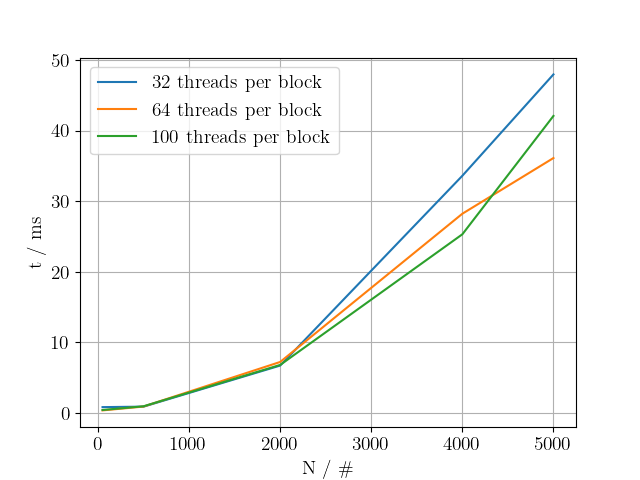
\includegraphics[width=0.5\textwidth]{../fig/lab3/step2.png}
    \caption{Runtime for $N \in \{50, 500, 2000, 4000, 5000\}$ and for 32, 64 and 100 threads per block respectively.}
    \label{fig:cuda_step2}
\end{figure}
\TODO{maybe add somethin, justification whatever?!}
\subsection{Step 3: Speedups}
We measure two different scenarios: 
\begin{enumerate}[i]
    \item excluding time of memory copy from CPU $\rightarrow$ GPU
    \item including time of memory copy from CPU $\rightarrow$ GPU
\end{enumerate}
After measuring \Shining{5} rounds without (i) and with (ii) memory access time we obtain the following \Shining{scatter plot} in \autoref{fig:cuda_step3}
\begin{figure}[H]
    \centering
    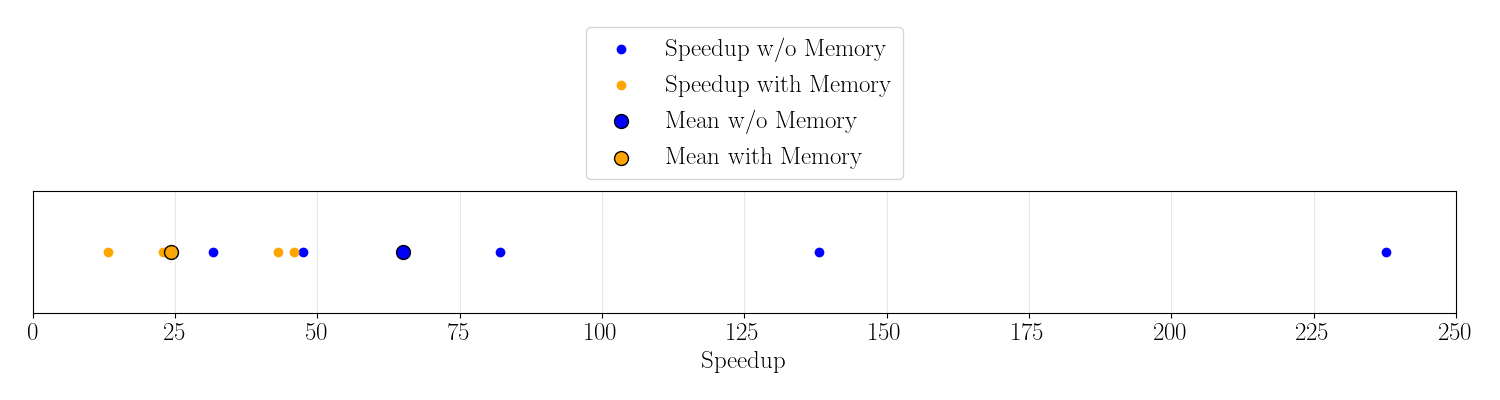
\includegraphics[width=\textwidth]{../fig/lab3/step3.png}
    \caption{Speedup of GPU implementation vs. CPU with and without memory transfer times.}
    \label{fig:cuda_step3}
\end{figure}
The mean speedup without memory access times is $\times 65$ and with memory access timed it comes out to $\times 24$.
\subsection{Step 4: Explanation of the results}

\newpage
\lstdefinelanguage{bash}{
  keywords={if, else, for, while, do, done, exit, then, fi, mkdir, echo, srun},
  keywordstyle=\color{blue}\bfseries,
  ndkeywords={sudo, cp, rm, touch, python3},
  ndkeywordstyle=\color{magenta}\bfseries,
  identifierstyle=\color{black},
  sensitive=false,
  comment=[l]{\#},
  morecomment=[s]{\#\#}{\#\#},
  commentstyle=\color{gray}\ttfamily,
  stringstyle=\color{darkgreen}\ttfamily,
  morestring=[b]",
  morestring=[b]'
}

\section*{Appendix - Introductory exercise}
\label{app:pingpong}
The following code was used for the ping pong task:
\lstinputlisting[language=c]{input/code/00/pingPong.c}
For the bonus task, the following code was used:
\lstinputlisting[language=c]{input/code/00/pingPongBonus.c}

\label{app:mm}
The matrix multiplication used the following code: 
\lstinputlisting[language=c]{../../01_lab0/src/MM-product.c}

\newpage
\section*{Appendix - Poisson solver}
\label{app:poisson}
The parallel Poisson solver used the following code:\\
\underline{Note:} Sbatch scripts used for the exercises will be included after the Poisson-solver code.\\
\lstinputlisting[language=c]{../../02_lab1/src/MPI_Poisson.c}
As an example for a launch-script for DB I'll present the following script used for \autoref{subsec:scaling} bellow. 
For a exhaustive reference of all scripts / files used go to \hrefu{https://github.com/etschgi1/HPC}{GitHub}.
\lstinputlisting[language=bash]{../../02_lab1/scripts/scaling_123.sh}

\newpage
\section*{Appendix - Finite elements simulation}
The following code was used to solve the tasks in \autoref{sec:fempois}:\\
\lstinputlisting[language=c]{../../03_lab2/src/MPI_Fempois.c}
An example of a sbatch script used for the timing of the finite elements simulation in \autoref{subsec:timing_fe} is shown bellow: 
\lstinputlisting[language=bash]{../../03_lab2/scripts/timing_22.sh}

\newpage
\section*{Appendix - Eigenvalue solution by Power Method on GPU}
The code for the CUDA assignment was mostly given and adapted in the main function and some kernels as detailed in \autoref{sec:ev}. The full code is given bellow: 
\lstinputlisting[language=c]{../../04_lab3/src/power_gpu.cu}

\end{document}